% ============================================================
%  Forces and Motion — Lesson Booklet (one section per lesson: A Reading · B Theory · C Practice · D Above level)
%  Years 7–8  |  Victorian Curriculum F–10 Version 2.0
%  Compile with: xelatex, three times (see CLAUDE.md) --- fill.py does this and sizes the answer boxes
%
%  TWO BUILDS FROM THIS ONE SOURCE (the Ch3G-L / Trebuchet pattern)
%    Forces_Motion_Lesson_Booklet_Yr7_8.tex          student copy --- no answers
%    Forces_Motion_Lesson_Booklet_Yr7_8_Teacher.tex  teacher copy --- defines
%        \teacheranswers (every \defans, read from teacher-answers/L01.tex ...
%        L14.tex, plus \teacherappendix) and then \input's this file, so every
%        box, cell, drawing space and graph prints its model answer in red.
%  The teacher wrapper, teacher-answers/ and the teacher PDF are gitignored:
%  answer keys never ship as a plain file (ROADMAP.md, "Staff material").
%  Keep this file free of answers. A key missing from the wrapper prints
%  ??key?? in the teacher copy, so grep the teacher PDF for "??" after a build.
%
%  Every answer-bearing piece of furniture carries a key: \abox{key}{h} (ruled
%  writing box), \wbox{key}{h} (plain box for calculations), \rcqk{key}{q}{h}
%  (comprehension Cn), \cell{key} (write-in table cell), \drawk{key}{h}{caption}
%  and \graphgrid{key}{h}. Keys were set from the printed numbering on
%  30 Oct 2026 (6.t3b = Task 6.3(b), 6.x9 = Extension 6.9, 6.c2 = C2,
%  6.wd1a = We do 6.1(a), 6.pred = prediction, 6.v3 = vocab row 3,
%  6.res-r2c3 = results table row 2 column 3) and are literal from then on:
%  renumbering the booklet never moves an answer. New furniture needs a new key.
%
%  Both copies paginate identically: answers sit inside fixed-height boxes and
%  cells. The teacher build reads the STUDENT page-fill file (.abx) and never
%  writes one, so build the student copy (and run fill.py) first. Both builds
%  log every key with its page and printed label to <jobname>.akp; the two
%  files must agree page for page (tools/forces_solutions.py checks this).
% ============================================================
\documentclass[11pt,a5paper,twoside]{article}
\newcommand{\unitname}{Forces and Motion}\newcommand{\unitcaps}{FORCES AND MOTION}

% ── Student / teacher switch ─────────────────────────────────────────────────
% The teacher wrapper defines \teacheranswers (every \defans) before \input-ing
% this file. Without it this is the student copy and every answer is blank.
\newif\ifteacher
\makeatletter
\newcommand{\defans}[2]{\@namedef{kans@#1}{#2}}
\newcommand{\getans}[1]{\@ifundefined{kans@#1}{\textbf{??#1??}}{\@nameuse{kans@#1}}}
\newcommand{\hasans}[1]{\@ifundefined{kans@#1}{\@secondoftwo}{\@firstoftwo}}
\makeatother
\ifdefined\teacheranswers \teachertrue \teacheranswers \fi
% Page-fill files always use the student copy's name, so the teacher build
% reads the student layout and never writes its own.
\providecommand\abbase{\jobname}

% ── Fonts (compile with XeLaTeX) ────────────────────────────────────────────
\usepackage{fontspec}
% Bundled fonts (in ./fonts/) so the document compiles anywhere with XeLaTeX/LuaLaTeX
\setmainfont{Lato}[                   % body — humanist sans (stands in for deck's Inter)
  Path=../fonts/, Extension=.ttf, Ligatures=TeX,
  UprightFont=Lato-Regular, ItalicFont=Lato-Italic,
  BoldFont=Lato-Bold, BoldItalicFont=Lato-BoldItalic ]
\newfontfamily\headingfont{Poppins}[  % display/headings — matches the slide decks
  Path=../fonts/, Extension=.ttf, Ligatures=TeX,
  UprightFont=Poppins-Regular, ItalicFont=Poppins-Italic,
  BoldFont=Poppins-Bold, BoldItalicFont=Poppins-BoldItalic ]
\setlength{\headheight}{22pt}

\usepackage[protrusion=true,expansion=false]{microtype}
\usepackage[a5paper, inner=17mm, outer=13mm, top=19mm, bottom=17mm, headheight=14pt, headsep=4mm, footskip=8mm]{geometry}
\usepackage{xcolor}
\usepackage{tikz}
\usetikzlibrary{arrows.meta, shapes.geometric, calc, positioning, decorations.pathreplacing}
\usepackage{tcolorbox}
\tcbuselibrary{skins, breakable, raster}
\usepackage{fancyhdr}
\usepackage{titlesec}
\usepackage{enumitem}
\usepackage{booktabs}
\usepackage{tabularx}
\usepackage{array}
\usepackage{colortbl}
\usepackage{multicol}
\usepackage{amsmath}
\usepackage{needspace}
% TikZ diagram macros are embedded below (just before \begin{document}) for easy editing.
\usepackage{longtable}
\usepackage{graphicx}
\usepackage{lastpage}
\usepackage{calc}
\usepackage{mdframed}
\usepackage{setspace}
\usepackage{ragged2e}
% PDF bookmarks: one per lesson (made in \sectiondiv) plus the cover and
% contents, and links from the contents table to each lesson.
% implicit=false: hyperref adds no anchors of its own (an anchor on each
% list item nudged lists down 1.5 mm, which would undo the page fill).
% hidelinks keeps the links invisible, so the printed pages are unchanged.
\usepackage[implicit=false, hidelinks,
  pdftitle={Forces and Motion — Lesson Booklet},
  pdfsubject={Years 7–8 Science, Victorian Curriculum F–10 v2.0}]{hyperref}
\usepackage{bookmark}
\makeatletter\providecommand\Hy@PageAnchorSlide{}\makeatother % writes the outline itself, which implicit=false switches off in hyperref

% ── Colour Palette ───────────────────────────────────────────────────────────
% Remapped to the slide-deck palette (names kept so body + diagrams cascade)
\definecolor{NavyBlue}   {HTML}{16305C}
\definecolor{MidBlue}    {HTML}{2E6FE0}
\definecolor{LightBlue}  {HTML}{E8F1FF}
\definecolor{TealGreen}  {HTML}{0F6E63}
\definecolor{LightGreen} {HTML}{E0F7F3}
\definecolor{GoldDark}   {HTML}{C77F12}
\definecolor{GoldLight}  {HTML}{FFF3DC}
\definecolor{PurpleDark} {HTML}{5B3FC0}
\definecolor{PurpleLight}{HTML}{EFE9FF}
\definecolor{OrangeDark} {HTML}{C9483D}
\definecolor{OrangeLight}{HTML}{FFE9E6}
\definecolor{MidGrey}    {HTML}{AEBED4}
\definecolor{LightGrey}  {HTML}{F2F5FA}
\definecolor{DarkGrey}   {HTML}{3A4759}
\definecolor{TableHead}  {HTML}{16305C}
\definecolor{RowAlt}     {HTML}{EEF4FF}
% Bright accent tints (deck) for bars, rules and chips
\definecolor{Blue}   {HTML}{2E6FE0}
\definecolor{Teal}   {HTML}{18A999}
\definecolor{Amber}  {HTML}{F5A623}
\definecolor{Coral}  {HTML}{FF6B5E}
\definecolor{Violet} {HTML}{7C5CE0}
\definecolor{Sky}    {HTML}{4DA3FF}
\definecolor{Ink}    {HTML}{16223A}
\definecolor{Line}   {HTML}{DDE5F0}
\definecolor{Paper}  {HTML}{FBFCFE}

% ── Page Style ───────────────────────────────────────────────────────────────
\pagestyle{fancy}
\fancyhf{}
\renewcommand{\headrulewidth}{0.4pt}
\renewcommand{\headrule}{\hbox to\headwidth{\color{NavyBlue}\leaders\hrule height \headrulewidth\hfill}}
\fancyhead[L]{\headingfont\small\color{NavyBlue}Forces and Motion}
\fancyhead[R]{\headingfont\small\ifteacher\textcolor{ScaffoldRed}{\bfseries Teacher copy}\ \textbar{}\ \fi\color{DarkGrey}Years 7--8 \textbar{} Victorian Curriculum F--10 v2.0}
\fancyfoot[C]{\headingfont\small\color{DarkGrey}\thepage\ \textbar{} \pageref{LastStudentPage}}
\fancypagestyle{plain}{%
  \fancyhf{}
  \fancyfoot[C]{\headingfont\small\color{DarkGrey}\thepage\ \textbar{} \pageref{LastStudentPage}}
  \renewcommand{\headrulewidth}{0pt}
}

% ── Section Formatting ───────────────────────────────────────────────────────
\titleformat{\section}
  {\headingfont\color{NavyBlue}\Large\bfseries}
  {}{0em}{}
  [{\color{Teal}\rule[0.6ex]{2.2em}{3pt}}{\color{Line}\rule[0.6ex]{\dimexpr\linewidth-2.2em\relax}{1pt}}]
\titlespacing{\section}{0pt}{18pt}{8pt}

\titleformat{\subsection}
  {\headingfont\color{MidBlue}\large\bfseries}
  {\thesubsection}{0.6em}{}
\titlespacing{\subsection}{0pt}{12pt}{4pt}

\titleformat{\subsubsection}
  {\headingfont\color{NavyBlue}\normalsize\bfseries}
  {}{0em}{}
\titlespacing{\subsubsection}{0pt}{8pt}{2pt}

% Deck-style eyebrow / kicker (optional use)
\newcommand{\kicker}[2][Teal]{%
  {\headingfont\bfseries\footnotesize\color{#1}%
   \textcolor{#1}{\rule[0.18ex]{1.6em}{2.2pt}}\hspace{0.5em}\MakeUppercase{#2}\par}%
  \vspace{2pt}}

% ── Custom tcolorbox Environments ────────────────────────────────────────────

% Section divider banner
\newtcolorbox{sectionbanner}[2]{
  enhanced, breakable=false,
  colback=NavyBlue, colframe=NavyBlue,
  fontupper=\color{white}\bfseries\large,
  left=4mm, right=4mm, top=3mm, bottom=3mm,
  title={\color{white}\Huge\bfseries #1},
  attach boxed title to top left={yshift=-2mm, xshift=4mm},
  boxed title style={colback=NavyBlue, colframe=NavyBlue},
  after upper={\par\smallskip\normalfont\normalsize\color{white!80!NavyBlue}\textit{#2}}
}

% Key info box (blue)
\newtcolorbox{infobox}[1]{
  breakable, arc=2.5mm, boxrule=0.5pt,
  colback=LightBlue, colframe=Blue!40,
  fonttitle=\headingfont\bfseries, coltitle=MidBlue,
  title={#1},
  left=4mm, right=3.5mm, top=2.5mm, bottom=2.5mm
}

% Scaffold box (yellow)
\newtcolorbox{scaffold}[1]{
  before upper={\anslabelset{Prediction}},
  breakable, arc=2.5mm, boxrule=0.5pt,
  colback=GoldLight, colframe=Amber!40,
  fonttitle=\headingfont\bfseries, coltitle=GoldDark,
  title={#1},
  left=4mm, right=3.5mm, top=2.5mm, bottom=2.5mm
}

% Worked example box
\newtcolorbox{workedexbox}[1]{
  breakable, arc=2.5mm, boxrule=0.5pt,
  colback=white, colframe=Amber!50,
  fonttitle=\headingfont\bfseries, coltitle=GoldDark,
  title={#1},
  left=4mm, right=3.5mm, top=2.5mm, bottom=2.5mm
}
% Worked examples: \begin{workedex}{title} -> "Worked Example N.M --- title",
% auto-numbered per section and labelled we:N.M. Never type the number.
\newcounter{wenum}[section]
\renewcommand{\thewenum}{\thesection.\arabic{wenum}}
\newenvironment{workedex}[1]
  {\refstepcounter{wenum}\label{we:\thewenum}\begin{workedexbox}{Worked Example \thewenum\ --- #1}}
  {\end{workedexbox}}

% We do: straight after each worked example, a near-identical question the
% class works through together, with its own writing space. Numbered to
% match the worked example above it and labelled wd:N.M.
%   \begin{wedo}{title} question ... \answerbox{h} \end{wedo}
\newtcolorbox{wedobox}[1]{
  enhanced, breakable=false, arc=2.5mm, boxrule=0.5pt,
  colback=white, colframe=TealGreen!55,
  fonttitle=\headingfont\bfseries, coltitle=TealGreen!75!black,
  title={#1},
  left=4mm, right=3.5mm, top=2.5mm, bottom=2.5mm
}
\newenvironment{wedo}[1]
  {\par\needspace{9\baselineskip}\anslabelset{We do \thewenum}\begin{wedobox}{We do \thewenum\ --- #1}\label{wd:\thewenum}\ignorespaces}
  {\end{wedobox}}

% Year 7 box (blue)
\newtcolorbox{yr7box}{
  breakable, arc=2.5mm, boxrule=0.5pt,
  colback=LightBlue, colframe=Blue!40,
  left=4mm, right=3.5mm, top=2.5mm, bottom=2.5mm
}

% Year 8 extension box (violet)
\newtcolorbox{yr8box}{
  breakable, arc=2.5mm, boxrule=0.5pt,
  colback=PurpleLight, colframe=Violet!40,
  left=4mm, right=3.5mm, top=2.5mm, bottom=2.5mm
}

% Answer lines box
\newcommand{\answerbox}[1]{%
  \begin{tcolorbox}[
    enhanced, breakable, arc=2mm,
    colback=Paper, colframe=Line,
    left=2mm, right=2mm, top=1mm, bottom=1mm,
    boxrule=1pt,
    height=#1
  ]
  \end{tcolorbox}%
}

% Experiment header
\newtcolorbox{expheader}[3]{
  breakable=false, arc=2.5mm,
  colback=RowAlt, colframe=Amber!50, boxrule=0.5pt,
  fonttitle=\headingfont\bfseries\large, coltitle=NavyBlue,
  title={Experiment #1: #2},
  left=4mm, right=3.5mm, top=2.5mm, bottom=2.5mm,
  after upper={\par\smallskip
    {\headingfont\bfseries\color{GoldDark}Aim:}\ \textit{#3}},
}

% Reading comprehension passage box (green)
\newtcolorbox{readingbox}[1]{
  breakable, arc=2.5mm, boxrule=0.5pt,
  colback=white, colframe=Teal!50,
  fonttitle=\headingfont\bfseries, coltitle=TealGreen,
  title={#1},
  left=4mm, right=3.5mm, top=2.5mm, bottom=2.5mm,
  fontupper=\normalsize
}

% Skill-builder box (for beginner scaffolding)
\newtcolorbox{skillbox}[1]{
  breakable, arc=2.5mm, boxrule=0.5pt,
  colback=RowAlt, colframe=Blue!40,
  fonttitle=\headingfont\bfseries, coltitle=MidBlue,
  title={#1},
  left=4mm, right=3.5mm, top=2.5mm, bottom=2.5mm
}

% ── Custom Commands ───────────────────────────────────────────────────────────

% Question: \question{marks}{text}  (marks can be empty)
% Numbered automatically as Q<section>.<n>, reset every section.
% Do NOT write numbers by hand.
\newcounter{qnum}[section]
\renewcommand{\theqnum}{\thesection.\arabic{qnum}}
\newcommand{\question}[2]{%
  \refstepcounter{qnum}%
  \needspace{3\baselineskip}%
  \medskip
  \noindent\label{q:\theqnum}\textbf{Q\theqnum}\ifx&#1&\else\ \textcolor{DarkGrey}{(#1 mark\ifnum#1=1\else s\fi)}\fi\quad #2%
  \medskip
}

% Inline marks note
\newcommand{\markscount}[1]{\hfill\textcolor{DarkGrey}{\textit{(#1 mark\ifnum#1=1\else s\fi)}}}

% ── Practice set counter and question macros ─────────────────────────────────
\newcounter{pqnum}
\newcommand{\practiceset}[1]{%
  \needspace{6\baselineskip}
  \setcounter{pqnum}{0}%
  \vspace{6pt}
  {\headingfont\bfseries\large\color{GoldDark} Practice Set --- #1}\\[-2pt]
  {\color{Amber}\rule{\linewidth}{1pt}}\\[2pt]
}
% \pq{question text}{working box height}
\newcommand{\pq}[2]{%
  \stepcounter{pqnum}%
  \needspace{4\baselineskip}
  \vspace{5pt}
  \noindent\textbf{\thepqnum.}\quad #1\par
  \vspace{2pt}
  \answerbox{#2}
}
% Two short questions side by side, each with its own box
\newcommand{\pqpair}[4]{%
  \needspace{4\baselineskip}
  \vspace{5pt}
  \noindent
  \begin{minipage}[t]{0.48\linewidth}
    \stepcounter{pqnum}\textbf{\thepqnum.}\quad #1\par\vspace{2pt}
    \begin{tcolorbox}[enhanced,arc=2mm,colback=Paper,colframe=Line,left=2mm,right=2mm,
      top=1mm,bottom=1mm,boxrule=1pt,height=#2]\end{tcolorbox}
  \end{minipage}\hfill
  \begin{minipage}[t]{0.48\linewidth}
    \stepcounter{pqnum}\textbf{\thepqnum.}\quad #3\par\vspace{2pt}
    \begin{tcolorbox}[enhanced,arc=2mm,colback=Paper,colframe=Line,left=2mm,right=2mm,
      top=1mm,bottom=1mm,boxrule=1pt,height=#4]\end{tcolorbox}
  \end{minipage}
}

% ── Comprehension question macro (compact, lined) ────────────────────────────
\newcounter{rcnum}
\newcommand{\rcreset}{\setcounter{rcnum}{0}}
\newcommand{\rcq}[2]{%
  \stepcounter{rcnum}%
  \needspace{3\baselineskip}
  \vspace{4pt}
  \noindent\textbf{C\thercnum.}\quad #1\par
  \vspace{2pt}
  \answerbox{#2}
}

% Section divider (big numbered banner): \sectiondiv{title}{summary}
%
% This IS the section: it steps the real section counter, so subsections,
% tasks, questions and figures inside it are numbered N.M automatically.
% Put \label{sec:N} straight after it. Never hand-type a section number.
\newcommand{\sectiondiv}[2]{%
  \needspace{5\baselineskip}%
  \refstepcounter{section}%
  % PDF bookmark for the lesson; its anchor, lesson.N.1, is what the contents table links to
  \pdfbookmark[1]{Lesson \thesection{} — #1}{lesson.\thesection}%
  \begin{tcolorbox}[
    enhanced, breakable=false, arc=3.5mm,
    colback=NavyBlue, colframe=NavyBlue, boxrule=0pt,
    sidebyside, sidebyside align=center,
    lefthand width=2.0cm,
    left=2mm, right=4mm, top=4mm, bottom=4mm
  ]
    \begin{center}
      {\headingfont\bfseries\color{white!35!NavyBlue}\fontsize{50}{50}\selectfont \thesection}
    \end{center}
    \tcblower
    {\headingfont\bfseries\color{white}\LARGE #1}\\[3pt]
    {\itshape\color{white!75!NavyBlue}\small #2}
  \end{tcolorbox}%
}

% Tasks: \task, \task[a] (part a of a NEW task), \taskpart{b} (next part
% of the same task), \exttask (Year 8 "Extension" — same counter).
% Numbered Task <section>.<n>, reset every section. Do NOT type numbers.
% Every task, question and figure also gets an automatic label
% (task:1.7b, q:2.4, fig:1.2, fig:E2.1) so page refs come from the .aux.
\newcounter{tasknum}[section]
\renewcommand{\thetasknum}{\thesection.\arabic{tasknum}}
\NewDocumentCommand{\task}{o}{\refstepcounter{tasknum}\label{task:\thetasknum\IfValueT{#1}{#1}}\textbf{Task \thetasknum\IfValueT{#1}{#1}}}
\newcommand{\taskpart}[1]{\label{task:\thetasknum#1}\textbf{Task \thetasknum#1}}
\newcommand{\exttask}{\refstepcounter{tasknum}\label{task:\thetasknum}\textbf{Extension \thetasknum}}

% Figure captions: \figcap[fig:label]{caption} -> "Figure N.M --- caption"
% \expfigcap{caption} -> "Figure EN.M" (experiment pages). Both auto-numbered.
\newcounter{fignum}[section]
\renewcommand{\thefignum}{\thesection.\arabic{fignum}}
\newcounter{expfignum}[section]
\renewcommand{\theexpfignum}{E\thesection.\arabic{expfignum}}
\newcommand{\figcap}[2][]{%
  \begin{center}
    \refstepcounter{fignum}\label{fig:\thefignum}\if\relax\detokenize{#1}\relax\else\label{#1}\fi
    \small\itshape\color{DarkGrey} Figure \thefignum\ --- #2
  \end{center}%
}
\newcommand{\expfigcap}[1]{%
  \begin{center}
    \refstepcounter{expfignum}\label{fig:\theexpfignum}%
    \small\itshape\color{DarkGrey} Figure \theexpfignum\ --- #1
  \end{center}%
}

% Diagram include
\newcommand{\diagramfig}[3]{%  {filename}{width fraction}{caption}
  \begin{center}
    \includegraphics[width=#2\linewidth]{#1}\\[4pt]
    \small\itshape\color{DarkGrey} #3
  \end{center}%
}

% Table column types
\newcolumntype{L}[1]{>{\RaggedRight\arraybackslash}p{#1}}
\newcolumntype{C}[1]{>{\Centering\arraybackslash}p{#1}}

% Table header colour
\newcommand{\thead}[1]{\cellcolor{TableHead}\color{white}\bfseries #1}
\newcommand{\talt}{\rowcolor{RowAlt}}
\newcommand{\tmid}{\rowcolor{MidGrey}}

% Inline year tags
\newcommand{\tagyr}[1]{%
  \tikz[baseline=-0.5ex]\node[
    rounded corners=2pt,
    fill=#1!20, draw=#1, text=#1,
    inner xsep=4pt, inner ysep=1pt,
    font=\scriptsize\bfseries
  ]{Yr #1 only};}

% Draw answer lines
\newcommand{\anslines}[1]{%
  \vspace{2pt}%
  \foreach \n in {1,...,#1}{%
    \par\noindent\rule{\linewidth}{0.3pt}\vspace{3pt}%
  }%
}

% ── Document ─────────────────────────────────────────────────────────────────
% ══════════════════════════════════════════════════════════════════════════════
%  EMBEDDED DIAGRAM DEFINITIONS  (formerly tikz_diagrams.tex)
%  Edit any figure here; each \diag... macro is called from the body by name.
% ══════════════════════════════════════════════════════════════════════════════
% ============================================================
%  TikZ Diagram Definitions — Forces and Motion Unit Booklet
%  Self-contained macros, no external image files.
%  Requires: tikz with arrows.meta, calc, positioning, patterns
% ============================================================

\usetikzlibrary{arrows.meta,calc,positioning,patterns,backgrounds}

\tikzset{
  force arrow/.style={-{Stealth[length=7pt,width=5pt]}, line width=2pt},
  dim arrow/.style={<->, >=Stealth, thin, color=DarkGrey},
  thin arrow/.style={-{Stealth[length=6pt,width=4pt]}, line width=1.4pt},
  ground hatch/.style={pattern=north east lines, pattern color=DarkGrey!50},
}

% ── D1: Contact vs Non-contact Forces ─────────────────────────────────────────
\newcommand{\diagForceTypes}{%
\begin{center}
\begin{fitbox}\begin{tikzpicture}[font=\small]
  % Contact forces box
  \node[draw=MidBlue, fill=LightBlue, rounded corners=5pt,
        minimum width=5.6cm, minimum height=3.8cm] (cbox) at (0,0) {};
  \node[font=\small\bfseries, text=NavyBlue] at (0, 1.65) {Contact Forces};
  \node[anchor=west, text=NavyBlue, font=\small] at (-2.5, 1.1)  {\textbullet\ Friction};
  \node[anchor=west, text=NavyBlue, font=\small] at (-2.5, 0.65) {\textbullet\ Normal force};
  \node[anchor=west, text=NavyBlue, font=\small] at (-2.5, 0.20) {\textbullet\ Tension};
  \node[anchor=west, text=NavyBlue, font=\small] at (-2.5,-0.25) {\textbullet\ Applied force};
  \node[anchor=west, text=NavyBlue, font=\small] at (-2.5,-0.70) {\textbullet\ Air resistance};
  \node[anchor=west, text=NavyBlue, font=\small] at (-2.5,-1.15) {\textbullet\ Spring force};
  % Non-contact forces box
  \node[draw=black!55!black, fill=black!8, rounded corners=5pt,
        minimum width=5.6cm, minimum height=3.8cm] (ncbox) at (6.4,0) {};
  \node[font=\small\bfseries, text=black!55!black] at (6.4, 1.65) {Non-contact Forces};
  \node[anchor=west, text=black!55!black, font=\small] at (3.9, 1.1)  {\textbullet\ Gravity};
  \node[anchor=west, text=black!55!black, font=\small] at (3.9, 0.65) {\textbullet\ Magnetic force};
  \node[anchor=west, text=black!55!black, font=\small] at (3.9, 0.20) {\textbullet\ Electrostatic force};
  \node[anchor=west, text=black!55!black, font=\small] at (3.9,-0.25) {\textbullet\ Nuclear force};
\end{tikzpicture}\end{fitbox}
\end{center}}

% ── D2: Free Body Diagrams ────────────────────────────────────────────────────
\newcommand{\diagFBD}{%
\begin{center}
\begin{fitbox}\begin{tikzpicture}[font=\small]
  % ── LEFT: Balanced ──
  \node[font=\small\bfseries, text=NavyBlue] at (0,3.6) {Balanced Forces};
  \fill[ground hatch] (-1.5,-1.0) rectangle (1.5,-0.7);
  \draw[thick, DarkGrey] (-1.5,-0.7) -- (1.5,-0.7);
  \node[draw=MidBlue, fill=LightBlue, rounded corners=3pt,
        minimum width=1.8cm, minimum height=1.0cm,
        font=\small\bfseries, text=NavyBlue] (book) at (0,0) {Book};
  % Normal up
  \draw[force arrow, TealGreen] (book.north) -- ++(0,1.8)
        node[right, font=\small\bfseries, text=TealGreen] {$N=10$\,N};
  % Weight down
  \draw[force arrow, black!65!black] (book.south) -- ++(0,-1.8)
        node[right, font=\small\bfseries, text=black!65!black] {$W=10$\,N};
  \node[font=\footnotesize\itshape, text=DarkGrey] at (0,-3.2) {Net force $= 0$\,N};
  \node[font=\footnotesize\itshape, text=DarkGrey] at (0,-3.65) {No acceleration};

  % ── RIGHT: Unbalanced ──
  \node[font=\small\bfseries, text=NavyBlue] at (7.5,3.6) {Unbalanced Forces};
  \fill[ground hatch] (6.0,-1.0) rectangle (9.0,-0.7);
  \draw[thick, DarkGrey] (6.0,-0.7) -- (9.0,-0.7);
  \node[draw=MidBlue, fill=LightBlue, rounded corners=3pt,
        minimum width=1.8cm, minimum height=1.0cm,
        font=\small\bfseries, text=NavyBlue] (box) at (7.5,0) {Box};
  % Normal up
  \draw[force arrow, TealGreen] (box.north) -- ++(0,1.8)
        node[right, font=\small\bfseries, text=TealGreen] {$N$};
  % Weight down
  \draw[force arrow, black!65!black] (box.south) -- ++(0,-1.8)
        node[right, font=\small\bfseries, text=black!65!black] {$W$};
  % Push right (20N, longer)
  \draw[force arrow, PurpleDark] (box.east) -- ++(2.6,0)
        node[above, font=\small\bfseries, text=PurpleDark] {Push 20\,N};
  % Friction left (5N, shorter)
  \draw[force arrow, OrangeDark] (box.west) -- ++(-1.6,0)
        node[above, font=\small\bfseries, text=OrangeDark] {Friction 5\,N};
  \node[font=\footnotesize\itshape, text=DarkGrey] at (7.5,-3.2) {Net force $= 15$\,N $\rightarrow$};
  \node[font=\footnotesize\itshape, text=DarkGrey] at (7.5,-3.65) {Accelerates rightward};
\end{tikzpicture}\end{fitbox}
\end{center}}

% ── D3: Newton's First Law ─────────────────────────────────────────────────────
\newcommand{\diagNewtonOne}{%
\begin{center}
\begin{fitbox}\begin{tikzpicture}[font=\small]
  % Law statement
  \node[draw=PurpleDark, fill=PurpleLight!50, rounded corners=5pt,
        minimum width=13cm, minimum height=1.1cm, align=center,
        font=\small\bfseries, text=PurpleDark] at (5.5,2.8)
        {\textit{``An object at rest stays at rest, and an object in motion stays in}\\[-1pt]
         \textit{motion, unless acted on by an unbalanced force.''\ (Law of Inertia)}};

  % Ground lines
  \draw[thick, DarkGrey] (-0.4,0) -- (2.2,0);
  \draw[thick, DarkGrey] (3.6,0) -- (7.0,0);
  \draw[thick, DarkGrey] (8.5,0) -- (11.5,0);

  % Ball 1: at rest
  \shade[ball color=MidBlue!80] (0.9,0.42) circle (0.42);
  \node[font=\footnotesize\bfseries, text=NavyBlue] at (0.9,1.9) {At rest};
  \draw[force arrow, TealGreen]   (0.9,0.84) -- (0.9,1.5);
  \draw[force arrow, black!65!black](0.9,0.0)  -- (0.9,-0.65);
  \node[font=\scriptsize, text=TealGreen, right]    at (0.9,1.2)  {$N$};
  \node[font=\scriptsize, text=black!65!black, right] at (0.9,-0.3) {$W$};
  \node[font=\scriptsize\itshape, text=DarkGrey] at (0.9,-1.1) {stays at rest};

  % Arrow 1→2
  \draw[-{Stealth}, thick, DarkGrey!60] (2.4,-2) -- (3.4,-2)
        node[midway, above, font=\scriptsize\itshape, text=DarkGrey] {no force added};

  % Ball 2: rolling
  \shade[ball color=TealGreen!70] (5.3,0.42) circle (0.42);
  \node[font=\footnotesize\bfseries, text=TealGreen] at (5.3,1.9) {Rolling (no friction)};
  \draw[force arrow, MidBlue] (5.72,0.42) -- (7.0,0.42)
        node[above, font=\scriptsize, text=MidBlue] {$v$};
  \node[font=\scriptsize\itshape, text=DarkGrey] at (5.3,-1.1) {keeps moving};

  % Arrow 2→3
  \draw[-{Stealth}, thick, DarkGrey!60] (7.4,-2) -- (8.3,-2)
        node[midway, above, font=\scriptsize\itshape, text=DarkGrey] {force applied};

  % Ball 3: stopping
  \shade[ball color=MidBlue!80] (9.9,0.42) circle (0.42);
  \node[font=\footnotesize\bfseries, text=black!60!black] at (9.9,1.9) {Unbalanced force};
  \draw[force arrow, black!65!black] (9.48,0.42) -- (8.4,0.42)
        node[above, font=\scriptsize, text=black!65!black] {friction};
  \node[font=\scriptsize\itshape, text=DarkGrey] at (9.9,-1.1) {decelerates / stops};
\end{tikzpicture}\end{fitbox}
\end{center}}

% ── D4: Newton's Second Law — F=ma ────────────────────────────────────────────
\newcommand{\diagFma}{%
\begin{center}
\begin{fitbox}\begin{tikzpicture}[font=\small]
  \node[draw=PurpleDark, fill=PurpleLight!50, rounded corners=5pt,
        minimum width=13cm, minimum height=0.9cm, align=center,
        font=\small\bfseries, text=PurpleDark]
        at (5.5,3.6)
        {Newton's Second Law: \quad $F = m \times a$ \quad $\Rightarrow$ \quad
         $a = F/m$ \quad $\Rightarrow$ \quad $m = F/a$};
  \node[draw=GoldDark, fill=GoldLight, rounded corners=5pt,
        minimum width=3.6cm, minimum height=3.2cm, align=center]
        at (0.8,1.5)
        {\textbf{\color{GoldDark}$F$\ (Force)}\\[4pt]
         \small\color{DarkGrey}Measured in newtons (N)\\
         \small\color{DarkGrey}A push or pull\\[2pt]
         \small\color{GoldDark}$F = m \times a$};
  \node[font=\large\bfseries, text=DarkGrey] at (3.3,1.5) {$=$};
  \node[draw=MidBlue, fill=LightBlue, rounded corners=5pt,
        minimum width=3.6cm, minimum height=3.2cm, align=center]
        at (5.5,1.5)
        {\textbf{\color{MidBlue}$m$\ (Mass)}\\[4pt]
         \small\color{DarkGrey}Measured in kg\\
         \small\color{DarkGrey}More mass\,=\,more\\
         \small\color{DarkGrey}inertia to overcome};
  \node[font=\large\bfseries, text=DarkGrey] at (7.75,1.5) {$\times$};
  \node[draw=TealGreen, fill=LightGreen, rounded corners=5pt,
        minimum width=3.6cm, minimum height=3.2cm, align=center]
        at (10.0,1.5)
        {\textbf{\color{TealGreen}$a$\ (Acceleration)}\\[4pt]
         \small\color{DarkGrey}Measured in m/s$^2$\\
         \small\color{DarkGrey}Bigger $F$ on same\\
         \small\color{DarkGrey}mass\,=\,bigger $a$};
\end{tikzpicture}\end{fitbox}
\end{center}}

% ── D5: Energy Types and Transformation ───────────────────────────────────────
\newcommand{\diagEnergy}{%
\begin{center}
\begin{fitbox}\begin{tikzpicture}[font=\small]
  % Top row: three energy type boxes
  \node[draw=GoldDark, fill=GoldLight, rounded corners=5pt,
        minimum width=4.0cm, minimum height=2.2cm, align=center]
        at (0.0,3.2)
        {\textbf{\color{GoldDark}Kinetic Energy (KE)}\\[3pt]
         \small\color{DarkGrey}Energy of motion\\[2pt]
         \small\color{GoldDark}$KE = \tfrac{1}{2}mv^2$};
  \node[draw=MidBlue, fill=LightBlue, rounded corners=5pt,
        minimum width=4.0cm, minimum height=2.2cm, align=center]
        at (4.8,3.2)
        {\textbf{\color{MidBlue}Gravitational PE}\\[3pt]
         \small\color{DarkGrey}Stored by height\\[2pt]
         \small\color{MidBlue}$GPE = mgh$};
  \node[draw=TealGreen, fill=LightGreen, rounded corners=5pt,
        minimum width=4.0cm, minimum height=2.2cm, align=center]
        at (9.6,3.2)
        {\textbf{\color{TealGreen}Elastic PE}\\[3pt]
         \small\color{DarkGrey}Stored by stretching\\[2pt]
         \small\color{DarkGrey}springs, rubber bands};
  % Divider label
  \node[font=\small\bfseries, text=DarkGrey] at (4.8,1.85)
        {Energy Transformation in a Trebuchet};
  % Chain: GPE box
  \node[draw=OrangeDark, fill=OrangeLight, rounded corners=4pt,
        minimum width=3.0cm, minimum height=1.1cm, align=center,
        font=\small\bfseries, text=OrangeDark] (n1) at (0.8,0.7)
        {Gravitational PE\\[-1pt]{\scriptsize\color{DarkGrey}(counterweight up)}};
  % Chain: KE1 box
  \node[draw=GoldDark, fill=GoldLight, rounded corners=4pt,
        minimum width=3.0cm, minimum height=1.1cm, align=center,
        font=\small\bfseries, text=GoldDark] (n2) at (4.8,0.7)
        {Kinetic Energy\\[-1pt]{\scriptsize\color{DarkGrey}(arm swings)}};
  % Chain: KE2 box
  \node[draw=TealGreen, fill=LightGreen, rounded corners=4pt,
        minimum width=3.0cm, minimum height=1.1cm, align=center,
        font=\small\bfseries, text=TealGreen] (n3) at (8.8,0.7)
        {Kinetic Energy\\[-1pt]{\scriptsize\color{DarkGrey}(ball launches)}};
  % Waste box
  \node[draw=DarkGrey, fill=LightGrey, rounded corners=4pt,
        minimum width=2.8cm, minimum height=0.9cm, align=center,
        font=\small, text=DarkGrey] (nw) at (8.8,-0.75)
        {$+$ Thermal \& Sound\\[-1pt]{\scriptsize(wasted)}};
  % Arrows
  \draw[-{Stealth}, thick, DarkGrey] (n1.east) -- (n2.west);
  \draw[-{Stealth}, thick, DarkGrey] (n2.east) -- (n3.west);
  \draw[-{Stealth}, thick, DarkGrey] (n3.south) -- (nw.north);
\end{tikzpicture}\end{fitbox}
\end{center}}

% ── D6: Three Classes of Lever ────────────────────────────────────────────────
\newcommand{\diagLevers}{%
\begin{center}
\begin{fitbox}\begin{tikzpicture}[font=\small]
  % ── Class 1: Fulcrum between E and L ── (effort and load both push down)
  \node[anchor=west, font=\small\bfseries, text=NavyBlue] at (-0.3,5.9) {Class 1: Fulcrum between E and L};
  \node[anchor=east, font=\small\itshape, text=DarkGrey]  at (12.0,5.9) {e.g.\ seesaw, crowbar};
  \draw[line width=4pt, DarkGrey!60, line cap=round] (1.0,4.2) -- (10.5,4.2);
  \fill[black!65!black] (5.5,4.2) -- ++(-.22,-.52) -- ++(.44,0) -- cycle;
  \node[font=\scriptsize\bfseries, text=black!65!black, right] at (5.75,3.9) {F};
  \draw[force arrow, MidBlue]   (1.5,5.05) -- (1.5,4.28);
  \draw[force arrow, TealGreen] (9.5,5.05) -- (9.5,4.28);
  \node[font=\small\bfseries, text=MidBlue,   above] at (1.5,5.05) {E};
  \node[font=\small\bfseries, text=TealGreen, above] at (9.5,5.05) {L};

  % ── Class 2: Load between F and E ── (effort lifts upwards)
  \node[anchor=west, font=\small\bfseries, text=NavyBlue] at (-0.3,3.25) {Class 2: Load between F and E};
  \node[anchor=east, font=\small\itshape, text=DarkGrey]  at (12.0,3.25) {e.g.\ wheelbarrow, nutcracker};
  \draw[line width=4pt, DarkGrey!60, line cap=round] (1.0,1.9) -- (10.5,1.9);
  \fill[black!65!black] (1.0,1.9) -- ++(-.22,-.52) -- ++(.44,0) -- cycle;
  \node[font=\scriptsize\bfseries, text=black!65!black, right] at (1.25,1.6) {F};
  \draw[force arrow, TealGreen] (5.0,2.75) -- (5.0,1.98);
  \node[font=\small\bfseries, text=TealGreen, above] at (5.0,2.75) {L};
  \draw[force arrow, MidBlue]   (9.5,1.0) -- (9.5,1.82);
  \node[font=\small\bfseries, text=MidBlue,   right] at (9.55,1.25) {E};

  % ── Class 3: Effort between F and L ── (effort lifts upwards)
  \node[anchor=west, font=\small\bfseries, text=NavyBlue] at (-0.3,0.35) {Class 3: Effort between F and L};
  \node[anchor=east, font=\small\itshape, text=DarkGrey]  at (12.0,0.35) {e.g.\ tweezers, your forearm};
  \draw[line width=4pt, DarkGrey!60, line cap=round] (1.0,-0.9) -- (10.5,-0.9);
  \fill[black!65!black] (1.0,-0.9) -- ++(-.22,-.52) -- ++(.44,0) -- cycle;
  \node[font=\scriptsize\bfseries, text=black!65!black, right] at (1.25,-1.2) {F};
  \draw[force arrow, TealGreen] (9.5,-0.05) -- (9.5,-0.82);
  \node[font=\small\bfseries, text=TealGreen, left] at (9.45,-0.3) {L};
  \draw[force arrow, MidBlue]   (5.0,-1.8) -- (5.0,-0.98);
  \node[font=\small\bfseries, text=MidBlue,   below] at (5.0,-1.8) {E};
\end{tikzpicture}\end{fitbox}
\end{center}}

% ── D7: Trebuchet as Class 1 Lever ────────────────────────────────────────────
\newcommand{\diagTrebuchetLever}{%
\begin{center}
\begin{fitbox}\begin{tikzpicture}[font=\small]
  % Ground
  \fill[ground hatch] (0,-0.55) rectangle (12.5,0);
  \draw[thick, DarkGrey] (0,0) -- (12.5,0);
  % A-frame holding the pivot
  \draw[line width=3pt, DarkGrey!70, line join=round] (4.9,0) -- (6.2,3.73) -- (7.5,0);
  % Arm (short end low on the left, long end high on the right)
  \draw[line width=6pt, black!55!black, line cap=round] (2.4,2.6) -- (10.5,5.0);
  % Pivot (fulcrum) sits on the arm
  \fill[DarkGrey!85] (6.2,3.73) circle (0.17);
  \node[font=\scriptsize\bfseries, text=DarkGrey, anchor=south east] at (6.05,3.95) {Pivot (fulcrum)};
  % Counterweight hangs from the short end
  \draw[thick, DarkGrey] (2.4,2.6) -- (2.4,1.95);
  \node[draw=black!60!black, fill=black!12, rounded corners=3pt,
        minimum width=1.9cm, minimum height=1.1cm,
        font=\small\bfseries, text=black!60!black, align=center]
        at (2.4,1.4) {Counterweight\\(effort)};
  \draw[force arrow, black!65!black] (2.4,0.85) -- (2.4,0.15);
  \node[font=\scriptsize, text=black!65!black, right] at (2.45,0.45) {$W$};
  % Projectile in the sling at the long end
  \shade[ball color=MidBlue!85] (10.9,5.2) circle (0.38);
  \node[font=\scriptsize\bfseries, text=MidBlue, anchor=west] at (11.35,5.2) {Projectile (load)};
  % Arm lengths
  \draw[dim arrow] (2.4,-0.95) -- (6.2,-0.95)
        node[midway, below, font=\scriptsize, text=black!60!black] {short arm (effort arm)};
  \draw[dim arrow] (6.2,-0.95) -- (10.5,-0.95)
        node[midway, below, font=\scriptsize, text=MidBlue] {long arm (load arm)};
  \draw[DarkGrey!45, densely dashed] (6.2,-1.1) -- (6.2,-0.6);
  \draw[DarkGrey!45, densely dashed] (10.5,-1.1) -- (10.5,4.7);
  \draw[DarkGrey!45, densely dashed] (2.4,-1.1) -- (2.4,-0.6);
  % MA formula box
  \node[draw=GoldDark, fill=GoldLight, rounded corners=3pt,
        font=\small, text=GoldDark, align=center, inner sep=4pt]
        at (6.2,-2.15)
        {$\text{MA} = \text{effort arm} \div \text{load arm} = \text{short arm} \div \text{long arm}$ \quad (less than 1)};
\end{tikzpicture}\end{fitbox}
\end{center}}

% ── D8: Projectile Motion ─────────────────────────────────────────────────────
\newcommand{\diagProjectile}{%
\begin{center}
\begin{fitbox}\begin{tikzpicture}[font=\small]
  % Ground
  \fill[ground hatch] (0,-0.45) rectangle (11.5,0);
  \draw[thick, DarkGrey] (0,0) -- (11.5,0);
  % Launch platform
  \fill[DarkGrey!35] (0,0) rectangle (1.3,3.0);
  \draw[thick, DarkGrey] (1.3,3.0) -- (0,3.0);
  % Height brace
  \draw[dim arrow] (-0.4,0) -- (-0.4,3.0)
        node[midway, left, font=\small\bfseries, text=black!65!black] {$h$};
  % Trajectory: launched sideways, so the path only ever curves down (a half parabola)
  \draw[thick, MidBlue, dashed] plot[domain=0:9.5, samples=60] ({1.3+\x},{3.0-0.033241*\x*\x});
  \node[font=\scriptsize\itshape, text=MidBlue, anchor=south west] at (6.9,2.05) {trajectory (a parabola)};
  % Ball at launch
  \shade[ball color=MidBlue!85] (1.3,3.0) circle (0.32);
  % Horizontal velocity
  \draw[force arrow, MidBlue] (1.62,3.0) -- (3.4,3.0)
        node[above, font=\small\bfseries, text=MidBlue] {$v$ (sideways)};
  % Weight at launch
  \draw[force arrow, black!65!black] (1.3,2.68) -- (1.3,1.4)
        node[right, font=\small\bfseries, text=black!65!black] {$W$};
  % Ball part-way: same sideways speed, same weight
  \shade[ball color=MidBlue!60] (5.3,2.468) circle (0.22);
  \draw[-{Stealth}, thick, MidBlue]       (5.52,2.468) -- ++(0.9,0);
  \draw[-{Stealth}, thick, black!65!black]  (5.3,2.248)  -- ++(0,-0.8)
        node[right, font=\scriptsize\bfseries, text=black!65!black] {$W$};
  % Ball at landing
  \shade[ball color=MidBlue!85] (10.8,0.32) circle (0.32);
  % Range brace
  \draw[dim arrow] (1.3,-0.75) -- (10.8,-0.75)
        node[midway, below, font=\small\bfseries, text=TealGreen] {$R$ (horizontal range)};
\end{tikzpicture}\end{fitbox}
\end{center}}

% ── New in this update: spring-scale and force-arrow scale diagrams ──────────
\newcommand{\diagSpringScales}{%
\begin{center}
\begin{fitbox}\begin{tikzpicture}[font=\footnotesize, x=.7cm, y=.7cm]
  % --- Scale A: 0-10 N, pointer at 4 N ---.
  \draw[line width=1pt, Ink] (0,0) rectangle (1.5,6);
  \node[font=\small\bfseries, text=Ink] at (0.75,6.35) {A};
  \draw[line width=1pt, Ink] (0.5,6) -- (0.5,6.5);
  \draw[line width=1pt, Ink] (0.75,-0.5) circle (0.22);
  \draw[line width=1pt, Ink] (0.75,0) -- (0.75,-0.28);
  \foreach \v in {0,1,2,3,4,5,6,7,8,9,10}{
    \pgfmathsetmacro{\yy}{5.5-\v*0.5}
    \draw[line width=0.7pt, Ink] (0.15,\yy) -- (0.55,\yy);
    \node[anchor=west, font=\tiny, text=DarkGrey] at (0.62,\yy) {\v};
  }
  \draw[line width=2pt, black!70!black] (0.1,3.5) -- (1.4,3.5);
  \node[anchor=west, font=\tiny\bfseries, text=black!70!black] at (1.5,3.5) {};
  \node[anchor=north, font=\tiny, text=DarkGrey] at (0.75,-0.85) {0--10\,N};

  % --- Scale B: 0-5 N, pointer at 2.5 N ---
  \begin{scope}[xshift=4cm]
    \draw[line width=1pt, Ink] (0,0) rectangle (1.5,6);
    \node[font=\small\bfseries, text=Ink] at (0.75,6.35) {B};
    \draw[line width=1pt, Ink] (0.5,6) -- (0.5,6.5);
    \draw[line width=1pt, Ink] (0.75,-0.5) circle (0.22);
    \draw[line width=1pt, Ink] (0.75,0) -- (0.75,-0.28);
    \foreach \v in {0,1,2,3,4,5}{
      \pgfmathsetmacro{\yy}{5.5-\v*1.0}
      \draw[line width=0.7pt, Ink] (0.15,\yy) -- (0.55,\yy);
      \node[anchor=west, font=\tiny, text=DarkGrey] at (0.62,\yy) {\v};
    }
    \foreach \v in {0.5,1.5,2.5,3.5,4.5}{
      \pgfmathsetmacro{\yy}{5.5-\v*1.0}
      \draw[line width=0.5pt, DarkGrey] (0.25,\yy) -- (0.45,\yy);
    }
    \draw[line width=2pt, black!70!black] (0.1,3.0) -- (1.4,3.0);
    \node[anchor=north, font=\tiny, text=DarkGrey] at (0.75,-0.85) {0--5\,N};
  \end{scope}

  % --- Scale C: 0-20 N, pointer at 13 N ---
  \begin{scope}[xshift=8cm]
    \draw[line width=1pt, Ink] (0,0) rectangle (1.5,6);
    \node[font=\small\bfseries, text=Ink] at (0.75,6.35) {C};
    \draw[line width=1pt, Ink] (0.5,6) -- (0.5,6.5);
    \draw[line width=1pt, Ink] (0.75,-0.5) circle (0.22);
    \draw[line width=1pt, Ink] (0.75,0) -- (0.75,-0.28);
    \foreach \v in {0,2,4,6,8,10,12,14,16,18,20}{
      \pgfmathsetmacro{\yy}{5.5-\v*0.25}
      \draw[line width=0.7pt, Ink] (0.15,\yy) -- (0.55,\yy);
      \node[anchor=west, font=\tiny, text=DarkGrey] at (0.62,\yy) {\v};
    }
    \draw[line width=2pt, black!70!black] (0.1,2.25) -- (1.4,2.25);
    \node[anchor=north, font=\tiny, text=DarkGrey] at (0.75,-0.85) {0--20\,N};
  \end{scope}

  % Instruction note
  \node[anchor=west, font=\footnotesize\itshape, text=DarkGrey, align=left]
        at (15.2,3) {Read the value where\\the red pointer sits.\\Check what one small\\division is worth first.};
\end{tikzpicture}\end{fitbox}
\end{center}}

% We do 1.1: one spring scale, 0-5 N with 20 small divisions, pointer on the 9th
\newcommand{\diagSpringScaleWeDo}{%
\begin{center}
\begin{fitbox}\begin{tikzpicture}[font=\footnotesize, x=0.8cm, y=0.8cm]
  \draw[line width=1pt, Ink] (0,0) rectangle (1.6,6);
  \draw[line width=1pt, Ink] (0.8,6) -- (0.8,6.5);
  \draw[line width=1pt, Ink] (0.8,6.65) circle (0.15);
  \draw[line width=1pt, Ink] (0.8,0) -- (0.8,-0.28);
  \draw[line width=1pt, Ink] (0.8,-0.5) circle (0.22);
  \foreach \i in {0,...,20}{
    \pgfmathsetmacro{\yy}{5.5-\i*0.25}
    \pgfmathtruncatemacro{\major}{mod(\i,4)==0}
    \ifnum\major=1
      \draw[line width=0.8pt, Ink] (0.12,\yy) -- (0.6,\yy);
      \pgfmathtruncatemacro{\lab}{\i/4}
      \node[anchor=west, font=\scriptsize, text=Ink] at (0.66,\yy) {\lab};
    \else
      \draw[line width=0.5pt, DarkGrey] (0.12,\yy) -- (0.38,\yy);
    \fi
  }
  \draw[line width=2pt, black!70!black] (0.05,3.25) -- (1.55,3.25);
  \draw[-{Stealth[length=2mm]}, black!70!black] (2.6,3.25) -- (1.7,3.25);
  \node[anchor=west, font=\scriptsize\bfseries, text=black!70!black] at (2.65,3.25) {pointer};
  \node[anchor=north, font=\scriptsize, text=DarkGrey] at (0.8,-0.85) {0--5\,N};
\end{tikzpicture}\end{fitbox}
\end{center}}

% ── Lesson 14: trajectories for one launch speed at five launch angles ───────
\newcommand{\diagRangeAngles}{%
\begin{center}
\begin{fitbox}\begin{tikzpicture}[font=\small, x=1.25cm, y=1.25cm]
  \fill[ground hatch] (-0.3,-0.3) rectangle (11.2,0);
  \draw[thick, DarkGrey] (-0.3,0) -- (11.2,0);
  % v = 10 m/s, g = 9.8: y = x tan(a) - 0.049 x^2 / cos^2(a)
  \foreach \a/\c/\r in {15/Amber/5.10, 30/TealGreen/8.84, 45/black!70!black/10.20, 60/MidBlue/8.84, 75/Violet/5.10}{
    \draw[thick, \c] plot[domain=0:\r, samples=60] (\x,{\x*tan(\a) - 0.049*\x*\x/(cos(\a)*cos(\a))});
  }
  \node[font=\scriptsize\bfseries, text=Amber]        at (2.55,0.58)  {15$^\circ$};
  \node[font=\scriptsize\bfseries, text=TealGreen]    at (4.42,1.52)  {30$^\circ$};
  \node[font=\scriptsize\bfseries, text=black!70!black] at (5.1,2.8)  {45$^\circ$};
  \node[font=\scriptsize\bfseries, text=MidBlue]      at (4.42,4.05) {60$^\circ$};
  \node[font=\scriptsize\bfseries, text=Violet]       at (2.55,5.0)  {75$^\circ$};
  \foreach \r/\lab in {5.10/5.1, 8.84/8.8, 10.20/10.2}{
    \draw[DarkGrey] (\r,0) -- (\r,-0.12);
    \node[font=\scriptsize, text=DarkGrey, below] at (\r,-0.12) {\lab\,m};
  }
  \node[font=\scriptsize\itshape, text=DarkGrey, anchor=west] at (0,-0.75) {All five balls are launched at 10\,m/s from ground level. Air resistance is ignored.};
\end{tikzpicture}\end{fitbox}
\end{center}}

\newcommand{\diagArrowScale}{%
\begin{center}
\begin{fitbox}\begin{tikzpicture}[font=\footnotesize, x=1cm, y=1cm]
  % Scale key
  \node[anchor=west, font=\small\bfseries, text=Ink] at (0,3.4) {Scale: 1\,cm represents 5\,N};
  \draw[line width=1.2pt, Ink] (0,3.0) -- (1,3.0);
  \draw[line width=0.8pt, Ink] (0,2.88) -- (0,3.12);
  \draw[line width=0.8pt, Ink] (1,2.88) -- (1,3.12);
  \node[anchor=west, font=\footnotesize, text=DarkGrey] at (1.2,3.0) {= 1\,cm = 5\,N};

  % 5 N arrow
  \draw[force arrow, MidBlue] (0,2.0) -- (1,2.0);
  \node[anchor=west, font=\footnotesize\bfseries, text=MidBlue] at (1.3,2.0) {5\,N \; (1\,cm long)};

  % 10 N arrow
  \draw[force arrow, TealGreen] (0,1.2) -- (2,1.2);
  \node[anchor=west, font=\footnotesize\bfseries, text=TealGreen] at (2.3,1.2) {10\,N \; (2\,cm long)};

  % 15 N arrow
  \draw[force arrow, OrangeDark] (0,0.4) -- (3,0.4);
  \node[anchor=west, font=\footnotesize\bfseries, text=OrangeDark] at (3.3,0.4) {15\,N \; (3\,cm long)};

  % Worked box on right
  \node[draw=GoldDark, fill=GoldLight, rounded corners=3pt, inner sep=5pt,
        font=\footnotesize, text=GoldDark, align=left, anchor=north west]
        at (8.2,3.3)
        {\textbf{To find the length:}\\[2pt]
         length $=$ force $\div$ scale\\[2pt]
         e.g.\ $15 \div 5 = 3$\,cm};
\end{tikzpicture}\end{fitbox}
\end{center}}


% ── Diagrams added with Lessons 4–6 (Newton's laws) ───────────────────────
% ── Newton's Third Law: two skaters, and a rocket with its exhaust ────────────
\newcommand{\diagThirdLaw}{%
\begin{center}
\begin{fitbox}\begin{tikzpicture}[font=\small]
  %% ── LEFT: two skaters push apart ──
  \node[font=\small\bfseries, text=NavyBlue] at (2.7,2.95) {Two skaters push apart};
  \fill[LightBlue] (0.3,-0.3) rectangle (5.1,0);
  \draw[thick, Sky] (0.3,0) -- (5.1,0);
  \node[font=\scriptsize\itshape, text=DarkGrey] at (2.7,-0.55) {ice};
  \node[draw=NavyBlue, fill=LightBlue, rounded corners=4pt,
        minimum width=1.4cm, minimum height=2.1cm,
        font=\small\bfseries, text=NavyBlue] (A) at (2.0,1.1) {A};
  \node[draw=TealGreen, fill=LightGreen, rounded corners=4pt,
        minimum width=1.4cm, minimum height=2.1cm,
        font=\small\bfseries, text=TealGreen] (B) at (3.4,1.1) {B};
  \draw[force arrow, OrangeDark] (A.west) -- ++(-1.3,0)
        node[above, font=\scriptsize\bfseries, text=OrangeDark, align=center] {B pushes A\\60\,N};
  \draw[force arrow, OrangeDark] (B.east) -- ++(1.3,0)
        node[above, font=\scriptsize\bfseries, text=OrangeDark, align=center] {A pushes B\\60\,N};

  %% ── RIGHT: a rocket in space and its exhaust gas ──
  \node[font=\small\bfseries, text=NavyBlue] at (11.0,2.95) {A rocket and its exhaust gas};
  % exhaust gas (drawn first)
  \shade[inner color=Amber!80, outer color=OrangeLight] (9.3,1.1) ellipse (0.6 and 0.42);
  \node[font=\scriptsize\bfseries, text=GoldDark] at (9.3,1.1) {gas};
  % fins
  \fill[NavyBlue!75] (9.95,1.45) -- (9.7,1.85) -- (10.35,1.45) -- cycle;
  \fill[NavyBlue!75] (9.95,0.75) -- (9.7,0.35) -- (10.35,0.75) -- cycle;
  % body and nose
  \draw[NavyBlue, fill=LightBlue, thick] (9.95,0.75) rectangle (11.75,1.45);
  \fill[NavyBlue] (11.75,0.75) -- (12.25,1.1) -- (11.75,1.45) -- cycle;
  \node[font=\scriptsize\bfseries, text=NavyBlue] at (10.9,1.1) {rocket};
  % the pair
  \draw[force arrow, OrangeDark] (8.7,1.1) -- ++(-1.3,0)
        node[above, font=\scriptsize\bfseries, text=OrangeDark, align=center] {rocket pushes\\gas back};
  \draw[force arrow, OrangeDark] (12.25,1.1) -- ++(1.3,0)
        node[above, font=\scriptsize\bfseries, text=OrangeDark, align=center] {gas pushes\\rocket forward};
  \node[font=\scriptsize\itshape, text=DarkGrey] at (10.8,-0.55) {in space --- no air needed};
\end{tikzpicture}\end{fitbox}
\end{center}}

% ── Newton's Second Law: formula triangle ──────────────────────────────────────
\newcommand{\diagFmaTriangle}{%
\begin{center}
\begin{fitbox}\begin{tikzpicture}[font=\small]
  \draw[thick, GoldDark, fill=GoldLight, line join=round] (0,0) -- (3.8,0) -- (1.9,3.0) -- cycle;
  \draw[thick, GoldDark] (0.76,1.2) -- (3.04,1.2);
  \draw[thick, GoldDark] (1.9,0) -- (1.9,1.2);
  \node[text=GoldDark]  at (1.9,1.85) {\LARGE $\boldsymbol{F}$};
  \node[text=MidBlue]   at (1.22,0.52) {\LARGE $\boldsymbol{m}$};
  \node[text=TealGreen] at (2.58,0.52) {\LARGE $\boldsymbol{a}$};
  \node[text=DarkGrey, fill=GoldLight, inner sep=1pt] at (1.9,0.52) {$\times$};
  % how to use it
  \node[anchor=west, align=left, text=Ink, font=\normalsize] at (4.8,1.5)
       {\textbf{Cover} $\boldsymbol{F}$:\quad $F = m \times a$\\[7pt]
        \textbf{Cover} $\boldsymbol{a}$:\quad $a = F \div m$\\[7pt]
        \textbf{Cover} $\boldsymbol{m}$:\quad $m = F \div a$};
  \node[anchor=west, align=left, text=DarkGrey, font=\footnotesize\itshape] at (4.8,-0.1)
       {Side by side means multiply. One above the other means divide.};
\end{tikzpicture}\end{fitbox}
\end{center}}


% ── Diagrams added with Lessons 7–9 (energy, bounce efficiency, levers) ────
% ── Sankey diagram: arrow width shows the amount of energy ───────────────────
\newcommand{\diagSankey}{%
\begin{center}
\begin{fitbox}\begin{tikzpicture}[font=\small]
  \node[font=\small\bfseries, text=NavyBlue, anchor=west] at (0,2.65)
       {An electric motor --- the width of each arrow shows how much energy};
  % energy in: 100 J (1 cm = 50 J)
  \fill[MidBlue!18] (0,0) rectangle (3,2);
  \draw[MidBlue, thick] (3,0) -- (0,0) -- (0,2) -- (3,2);
  \node[align=center, text=NavyBlue] at (1.5,1.0) {Electrical\\energy in\\\textbf{100\,J}};
  % useful: 70 J, carries straight on
  \fill[TealGreen!22] (3,0.6) -- (7.4,0.6) -- (7.4,0.3) -- (8.4,1.3) -- (7.4,2.3) -- (7.4,2.0) -- (3,2.0) -- cycle;
  \draw[TealGreen, thick] (3,2.0) -- (7.4,2.0) -- (7.4,2.3) -- (8.4,1.3) -- (7.4,0.3) -- (7.4,0.6) -- (4.4,0.6);
  \node[align=center, text=TealGreen] at (5.6,1.3) {\textbf{Useful:} kinetic energy\\\textbf{70\,J}};
  % wasted: 30 J, turns downwards
  \fill[OrangeDark!18] (3,0) arc[start angle=90, end angle=0, radius=0.8] -- (3.8,-1.3) -- (3.55,-1.3)
        -- (4.1,-2.0) -- (4.65,-1.3) -- (4.4,-1.3) -- (4.4,-0.8) arc[start angle=0, end angle=90, radius=1.4] -- cycle;
  \draw[OrangeDark, thick] (3,0) arc[start angle=90, end angle=0, radius=0.8] -- (3.8,-1.3) -- (3.55,-1.3)
        -- (4.1,-2.0) -- (4.65,-1.3) -- (4.4,-1.3) -- (4.4,-0.8) arc[start angle=0, end angle=90, radius=1.4];
  \node[align=left, text=OrangeDark, anchor=west] at (4.9,-1.35) {\textbf{Wasted:} thermal energy and sound\\\textbf{30\,J}};
\end{tikzpicture}\end{fitbox}
\end{center}}

% ── Experiment 3: measuring drop height and bounce height ────────────────────
\newcommand{\diagBounceSetup}{%
\begin{center}
\begin{fitbox}\begin{tikzpicture}[font=\small, y=1cm]
  % floor and wall
  \fill[ground hatch] (-0.6,-0.3) rectangle (8.8,0);
  \draw[thick, DarkGrey] (-0.6,0) -- (8.8,0);
  \fill[ground hatch] (-0.6,0) rectangle (-0.3,4.5);
  \draw[thick, DarkGrey] (-0.3,0) -- (-0.3,4.5);
  % metre rulers taped to the wall: 1 unit = 40 cm
  \fill[GoldLight] (-0.3,0) rectangle (0.25,4.2);
  \draw[GoldDark] (-0.3,0) rectangle (0.25,4.2);
  \foreach \y in {0,0.25,...,4.0} \draw[GoldDark] (0.25,\y) -- (0.12,\y);
  \foreach \y/\l in {0/0,1/40,2/80,3/120,4/160} {
    \draw[GoldDark, thick] (0.25,\y) -- (0.0,\y);
    \node[font=\scriptsize, text=GoldDark, anchor=east] at (-0.32,\y) {\l};
  }
  \node[font=\scriptsize\itshape, text=GoldDark, rotate=90] at (-1.45,2.1) {height (cm)};
  % ball before release (bottom of ball at 120 cm)
  \shade[ball color=Amber!80] (1.5,3.25) circle (0.25);
  \draw[dotted, DarkGrey] (0.25,3.0) -- (1.5,3.0);
  % path of the ball
  \draw[dashed, DarkGrey!70, -{Stealth}] (1.5,2.95) -- (2.4,0.55);
  \shade[ball color=Amber!80] (2.55,0.25) circle (0.25);
  \draw[dashed, DarkGrey!70, -{Stealth}] (2.7,0.55) -- (3.45,1.6);
  \shade[ball color=Amber!80] (3.6,1.9) circle (0.25);
  \draw[dotted, DarkGrey] (0.25,1.65) -- (3.6,1.65);
  % heights
  \draw[dim arrow] (7.0,0) -- (7.0,3.0) node[midway, right, font=\small, text=NavyBlue] {drop height $h_1$};
  \draw[dim arrow] (4.4,0) -- (4.4,1.65) node[midway, right, font=\small, text=TealGreen] {bounce height $h_2$};
  \draw[DarkGrey!60] (1.75,3.0) -- (7.2,3.0);
  \draw[DarkGrey!60] (3.85,1.65) -- (4.6,1.65);
  % reading tip
  \node[font=\scriptsize\itshape, text=DarkGrey, align=left, anchor=west] at (1.9,4.05)
       {Read the \textbf{bottom} of the ball, at eye level\\(or film it in slow motion and pause at the top).};
\end{tikzpicture}\end{fitbox}
\end{center}}

% ── Parts of a lever: fulcrum, effort, load and the two arms ─────────────────
\newcommand{\diagLeverParts}{%
\begin{center}
\begin{fitbox}\begin{tikzpicture}[font=\small]
  % beam
  \draw[line width=5pt, DarkGrey!60, line cap=round] (0.4,1.0) -- (10.2,1.0);
  % fulcrum
  \fill[black!65!black] (3.4,0.88) -- (3.0,0.2) -- (3.8,0.2) -- cycle;
  \node[font=\small\bfseries, text=black!65!black] at (3.4,-0.1) {Fulcrum (pivot)};
  % load on the short side
  \node[draw=TealGreen, fill=LightGreen, rounded corners=3pt, minimum width=1.3cm, minimum height=0.9cm,
        font=\small\bfseries, text=TealGreen] at (1.0,1.6) {Load};
  % effort on the long side
  \draw[force arrow, MidBlue] (9.6,2.6) -- (9.6,1.15);
  \node[font=\small\bfseries, text=MidBlue, above] at (9.6,2.6) {Effort (your push)};
  % arms
  \draw[dim arrow] (1.0,-0.65) -- (3.4,-0.65) node[midway, below, font=\small, text=TealGreen] {load arm};
  \draw[dim arrow] (3.4,-0.65) -- (9.6,-0.65) node[midway, below, font=\small, text=MidBlue] {effort arm};
  \draw[DarkGrey!50] (1.0,0.85) -- (1.0,-0.8);
  \draw[DarkGrey!50] (9.6,0.85) -- (9.6,-0.8);
\end{tikzpicture}\end{fitbox}
\end{center}}


% ── Diagrams added with Lessons 10–12 (Experiment 4, levers extension, projectiles) ──
% ── Experiment 4: a metre stick balanced on a fulcrum at the 50 cm mark ──────
%    1 unit = 1/0.12 cm of stick, so the 0–100 cm stick runs from x = 0 to 12.
\newcommand{\diagExpFourSetup}{%
\begin{center}
\begin{fitbox}\begin{tikzpicture}[font=\small, x=1.2cm, y=1cm]
  % bench
  \fill[ground hatch] (-0.3,0.15) rectangle (12.3,0.5);
  \draw[thick, DarkGrey] (-0.3,0.5) -- (12.3,0.5);
  \node[font=\scriptsize\itshape, text=DarkGrey, anchor=west] at (-0.25,0.3) {bench};
  % fulcrum: triangular prism under the 50 cm mark
  \fill[black!65!black] (6.0,1.5) -- (5.6,0.5) -- (6.4,0.5) -- cycle;
  \node[font=\small\bfseries, text=black!65!black, anchor=west] at (6.5,0.95) {fulcrum at 50\,cm};
  % metre stick, with a scale every 10 cm
  \draw[fill=GoldLight, draw=GoldDark] (0,1.5) rectangle (12,1.9);
  \foreach \c in {0,10,...,100} {
    \draw[GoldDark] ({0.12*\c},1.9) -- ({0.12*\c},1.76);
  }
  \foreach \c in {5,15,...,95} { \draw[GoldDark!70] ({0.12*\c},1.9) -- ({0.12*\c},1.82); }
  \foreach \c in {10,20,30,40,60,70,80,90} {
    \node[font=\scriptsize, text=GoldDark] at ({0.12*\c},1.63) {\c};
  }
  \node[font=\scriptsize\itshape, text=GoldDark, anchor=north west] at (0.1,1.45) {metre stick};
  % load: 100 g standing on the 30 cm mark
  \draw[fill=TealGreen!25, draw=TealGreen, rounded corners=1pt] (3.25,1.9) rectangle (3.95,2.75);
  \node[font=\small\bfseries, text=TealGreen] at (3.6,2.325) {100\,g};
  \node[font=\small\bfseries, text=TealGreen] at (3.6,3.05) {Load};
  % effort: one 50 g slotted mass on the 90 cm mark
  \draw[fill=MidBlue!25, draw=MidBlue, rounded corners=1pt] (10.5,1.9) rectangle (11.1,2.32);
  \node[font=\scriptsize\bfseries, text=MidBlue] at (10.8,2.11) {50\,g};
  \node[font=\small\bfseries, text=MidBlue] at (10.8,2.62) {Effort};
  % arms, measured from the fulcrum to the centre of each mass
  \draw[densely dashed, DarkGrey!60] (3.6,3.3) -- (3.6,3.95);
  \draw[densely dashed, DarkGrey!60] (6.0,1.9) -- (6.0,3.95);
  \draw[densely dashed, DarkGrey!60] (10.8,2.87) -- (10.8,3.95);
  \draw[dim arrow] (3.6,3.8) -- (6.0,3.8) node[midway, above, font=\small, text=TealGreen] {load arm = 20\,cm};
  \draw[dim arrow] (6.0,3.8) -- (10.8,3.8) node[midway, above, font=\small, text=MidBlue] {effort arm = 40\,cm};
\end{tikzpicture}\end{fitbox}
\end{center}}

% ── Same angle, different arcs: why the long end of an arm moves faster ──────
\newcommand{\diagArmArcs}{%
\begin{center}
\begin{fitbox}\begin{tikzpicture}[font=\small]
  \def\ang{50}
  % starting position of the arm (faint)
  \draw[line width=4pt, DarkGrey!25, line cap=round] (-1.2,0) -- (4.8,0);
  % turned position of the arm
  \draw[line width=4pt, black!55!black, line cap=round] ({-1.2*cos(\ang)},{-1.2*sin(\ang)}) -- ({4.8*cos(\ang)},{4.8*sin(\ang)});
  % arcs travelled by each end in the same time
  \draw[very thick, MidBlue, -{Stealth[length=8pt,width=6pt]}] (4.8,0) arc[start angle=0, end angle=\ang, radius=4.8];
  \draw[very thick, black!65!black, -{Stealth[length=7pt,width=5pt]}] (-1.2,0) arc[start angle=180, end angle={180+\ang}, radius=1.2];
  % pivot
  \fill[DarkGrey] (0,0) circle (0.12);
  \node[font=\scriptsize\bfseries, text=DarkGrey, anchor=north] at (0.25,-0.15) {pivot};
  % angle mark
  \draw[DarkGrey] (0.8,0) arc[start angle=0, end angle=\ang, radius=0.8];
  \node[font=\scriptsize, text=DarkGrey, anchor=west] at ({0.9*cos(14)},{0.9*sin(14)}) {same angle};
  % labels
  \node[font=\small\bfseries, text=MidBlue, anchor=west, align=left] at (5.0,1.8)
       {long arm: big arc\\in the same time \(\rightarrow\) fast};
  \node[font=\small\bfseries, text=black!65!black, anchor=east, align=right] at (-1.35,-0.75)
       {short arm: small arc\\\(\rightarrow\) slow};
\end{tikzpicture}\end{fitbox}
\end{center}}

% ── Two independent motions: a dropped ball and a ball launched sideways ──────
%    h = 1.25 m, launch speed 3.0 m/s, positions every 0.1 s (1 m = 4.4 units)
\newcommand{\diagTwoMotions}{%
\begin{center}
\begin{fitbox}\begin{tikzpicture}[font=\small, x=1cm, y=1cm]
  \fill[ground hatch] (-1.4,-0.3) rectangle (8.6,0);
  \draw[thick, DarkGrey] (-1.4,0) -- (8.6,0);
  \foreach \t in {0,1,2,3,4} {
    \pgfmathsetmacro{\yy}{5.5-4.4*4.9*(\t/10)*(\t/10)}
    \pgfmathsetmacro{\xx}{1.2+4.4*3.0*(\t/10)}
    \draw[densely dashed, DarkGrey!45] (-0.4,\yy) -- (8.4,\yy);
    \ifnum\t>0 \node[font=\scriptsize, text=DarkGrey, anchor=east] at (-0.45,\yy) {0.\t\,s};\fi
    \shade[ball color=black!70] (0,\yy) circle (0.11);
    \shade[ball color=MidBlue!85] (\xx,\yy) circle (0.11);
  }
  % path of the launched ball
  \draw[MidBlue, thin, dashed] plot[domain=0:0.505, samples=40] ({1.2+13.2*\x},{5.5-21.56*\x*\x});
  % both land at t = 0.505 s
  \shade[ball color=black!70] (0,0.11) circle (0.11);
  \shade[ball color=MidBlue!85] ({1.2+13.2*0.505},0.11) circle (0.11);
  \node[font=\scriptsize, text=DarkGrey, anchor=east] at (-0.45,0.15) {0.51\,s};
  % labels
  \node[font=\small\bfseries, text=black!65!black, anchor=south] at (0,5.7) {dropped};
  \node[font=\small\bfseries, text=MidBlue, anchor=south west] at (1.0,5.7) {launched sideways at 3\,m/s};
  \draw[thin arrow, MidBlue] (1.4,5.5) -- (2.15,5.5);
\end{tikzpicture}\end{fitbox}
\end{center}}

% ── Optional-lesson note, shown under the lesson banner ──────────────────────
\newcommand{\optionalnote}[1]{%
  % the title is a bold lead-in on the first line rather than a title bar,
  % which keeps Lesson 11's reading on the lesson's first page
  \begin{tcolorbox}[enhanced, breakable=false, arc=2.5mm, boxrule=0.5pt,
    colback=PurpleLight, colframe=Violet!50,
    left=4mm, right=3.5mm, top=2mm, bottom=2mm]
  {\headingfont\bfseries\color{PurpleDark}Optional lesson \textbullet{} Year 8 extension.}\enspace #1
  \end{tcolorbox}\vspace{2pt}}


% ── Motion sensor set-up for Experiment 5 ────────────────────────────────────
\newcommand{\diagMotionSensorSetup}{%
\begin{center}
\begin{fitbox}\begin{tikzpicture}[font=\small, x=1cm, y=0.74cm]
  % floor
  \fill[ground hatch] (-0.4,-0.3) rectangle (10.2,0);
  \draw[thick, DarkGrey] (-0.4,0) -- (10.2,0);
  % bench, its right-hand edge at x = 4
  \fill[LightGrey, draw=DarkGrey] (-0.2,3.25) rectangle (4.0,3.45);
  \fill[DarkGrey!70] (0.0,0) rectangle (0.15,3.25);
  \fill[DarkGrey!70] (3.7,0) rectangle (3.85,3.25);
  \node[font=\scriptsize\itshape, text=DarkGrey] at (2.0,3.05) {bench};
  % data logger on the bench
  \draw[fill=white, draw=DarkGrey, rounded corners=1pt] (0.3,3.45) rectangle (1.9,4.45);
  \draw[MidBlue, thick] (0.45,3.62) -- (0.75,3.62) -- (1.45,4.25) -- (1.52,3.62) -- (1.75,3.62);
  \node[font=\scriptsize\itshape, text=DarkGrey, anchor=south] at (1.1,4.45) {data logger};
  % stand: base, upright rod, right-angle clamp and an arm reaching over the edge
  \fill[DarkGrey] (2.4,3.45) rectangle (3.6,3.62);
  \draw[line width=2.2pt, DarkGrey!80] (3.0,3.62) -- (3.0,6.95);
  \draw[line width=2.2pt, DarkGrey!80] (3.0,6.6) -- (5.7,6.6);
  \fill[DarkGrey] (2.86,6.46) rectangle (3.14,6.74);
  \node[font=\scriptsize\itshape, text=DarkGrey, anchor=east] at (2.85,6.1) {stand};
  % motion sensor, pointing straight down
  \draw[fill=NavyBlue, draw=NavyBlue, rounded corners=2pt] (5.15,6.0) rectangle (6.25,6.75);
  \fill[MidGrey] (5.3,5.96) rectangle (6.1,6.06);
  \node[font=\small\bfseries, text=NavyBlue, anchor=west] at (6.45,7.3) {motion sensor};
  \node[font=\scriptsize\itshape, text=DarkGrey, anchor=north west, align=left] at (6.45,7.0)
       {sends pulses of sound down\\and times their echoes};
  % cable to the logger
  \draw[DarkGrey!70, thick] (5.15,6.4) .. controls (4.2,6.2) and (2.4,5.2) .. (1.9,4.1);
  % sound pulses
  \foreach \r in {0.25,0.45,0.65} {
    \draw[MidBlue!70, thick] ($(5.7,5.96)+(-130:\r)$) arc[start angle=-130, end angle=-50, radius=\r];
  }
  % the weight, held with its bottom 40 cm below the sensor
  \draw[fill=MidGrey!70, draw=DarkGrey] (5.35,4.4) rectangle (6.05,4.95);
  \draw[fill=MidGrey!40, draw=DarkGrey] (5.7,4.95) ellipse (0.35 and 0.09);
  \node[font=\scriptsize\bfseries, text=DarkGrey, anchor=west] at (6.15,4.68) {weight};
  \draw[dim arrow] (4.95,5.96) -- (4.95,4.4) node[midway, left, font=\small, text=DarkGrey] {40\,cm};
  \draw[densely dashed, DarkGrey!50] (4.85,4.4) -- (5.3,4.4);
  \draw[densely dashed, DarkGrey!50] (4.85,5.96) -- (5.15,5.96);
  % its fall
  \draw[densely dashed, TealGreen, -{Stealth[length=6pt]}] (5.7,4.3) -- (5.7,0.55);
  \node[font=\scriptsize\itshape, text=TealGreen, anchor=west] at (5.8,2.4) {falls};
  % cushion
  \draw[fill=GoldLight, draw=GoldDark, rounded corners=3pt] (4.8,0) rectangle (6.6,0.32);
  \node[font=\scriptsize\itshape, text=GoldDark, anchor=west] at (6.7,0.2) {cushion (no-bounce pad)};
\end{tikzpicture}\end{fitbox}
\end{center}}

% ── A velocity–time graph for one drop under the motion sensor ───────────────
% \diagVelocityTime{numbers} labels the axes with values (Lesson 12);
% \diagVelocityTime{parts} labels what each part of the line means (Lesson 13).
\newcommand{\diagVelocityTime}[1]{%
\begin{center}
\begin{fitbox}\begin{tikzpicture}[font=\small, x=11cm, y=0.8cm]
  % grid and axes: time 0–0.7 s, velocity 0–5 m/s
  \foreach \t in {0.1,0.2,...,0.71} \draw[Line] (\t,0) -- (\t,5);
  \foreach \v in {1,...,5} \draw[Line] (0,\v) -- (0.7,\v);
  \draw[thick, DarkGrey, -{Stealth[length=6pt]}] (0,0) -- (0.73,0) node[right, font=\small, text=DarkGrey] {time (s)};
  \draw[thick, DarkGrey, -{Stealth[length=6pt]}] (0,0) -- (0,5.4) node[above, font=\small, text=DarkGrey] {velocity (m/s)};
  \foreach \t/\l in {0/0,0.1/0.1,0.2/0.2,0.3/0.3,0.4/0.4,0.5/0.5,0.6/0.6,0.7/0.7} \node[font=\scriptsize, text=DarkGrey, below] at (\t,0) {\l};
  \foreach \v in {0,...,5} \node[font=\scriptsize, text=DarkGrey, left] at (0,\v) {\v};
  % the line: held still, falling, landing
  \draw[line width=1.6pt, MidBlue] (0,0) -- (0.10,0) -- (0.55,4.4) -- (0.565,0.05) -- (0.7,0.05);
  \fill[TealGreen] (0.10,0) circle (2pt);
  \fill[OrangeDark] (0.55,4.4) circle (2pt);
  \def\vtmode{#1}\def\vtnumbers{numbers}%
  \ifx\vtmode\vtnumbers
    \draw[densely dashed, DarkGrey!60] (0,4.4) -- (0.55,4.4);
    \draw[densely dashed, DarkGrey!60] (0.55,0) -- (0.55,4.4);
    \node[font=\scriptsize\bfseries, text=TealGreen, anchor=south east, align=right] at (0.10,0.15) {let go\\0\,m/s};
    \node[font=\scriptsize\bfseries, text=OrangeDark, anchor=west, align=left] at (0.565,4.4) {just before\\it lands: 4.4\,m/s};
  \else
    \node[font=\scriptsize, text=DarkGrey, align=center, anchor=south] at (0.05,0.2) {held\\still};
    \node[font=\scriptsize\bfseries, text=TealGreen, anchor=north west, align=left] at (0.11,-0.45) {starting velocity\\(the moment it is let go)};
    \node[font=\scriptsize\bfseries, text=OrangeDark, anchor=west, align=left] at (0.565,4.4) {final velocity\\(just before it lands)};
    \node[font=\scriptsize, text=MidBlue, anchor=north west, align=left, fill=white, inner sep=1.5pt] at (0.03,4.75) {falling: a straight line, because\\the speed goes up steadily};
    \draw[MidBlue, -{Stealth[length=4pt]}] (0.16,3.9) -- (0.29,2.05);
    \node[font=\scriptsize, text=DarkGrey, anchor=west, align=left] at (0.58,0.9) {lands on\\the cushion};
    \draw[dim arrow] (0.10,-1.35) -- (0.55,-1.35) node[midway, below, font=\scriptsize, text=DarkGrey] {time of fall};
    \draw[densely dashed, DarkGrey!50] (0.10,-0.5) -- (0.10,-1.45);
    \draw[densely dashed, DarkGrey!50] (0.55,-0.5) -- (0.55,-1.45);
  \fi
\end{tikzpicture}\end{fitbox}
\end{center}}

% ── Experiment 2: pulling a loaded wooden block along the bench with a spring balance ──
\newcommand{\diagExpTwoSetup}{%
\begin{center}
\begin{fitbox}\begin{tikzpicture}[font=\small, x=1.18cm, y=1.18cm]
  % bench
  \fill[ground hatch] (0,-0.35) rectangle (13,0);
  \draw[thick, DarkGrey] (0,0) -- (13,0);
  \node[font=\scriptsize\itshape, text=DarkGrey, anchor=west] at (0.05,-0.18) {bench top};
  % wooden block with a hook on its left face
  \draw[fill=GoldLight, draw=GoldDark, thick] (7.2,0) rectangle (10.2,1.3);
  \foreach \y in {0.35,0.7,1.0} { \draw[GoldDark!45] (7.35,\y) .. controls (8.2,\y+0.08) and (9.2,\y-0.08) .. (10.05,\y); }
  \draw[DarkGrey, thick] (7.2,0.65) -- (6.95,0.65);
  \draw[DarkGrey, thick] (6.85,0.65) circle (0.1);
  % two 200 g slotted masses on top
  \draw[fill=MidBlue!22, draw=MidBlue, thick, rounded corners=1pt] (7.9,1.3) rectangle (9.5,1.62);
  \draw[fill=MidBlue!22, draw=MidBlue, thick, rounded corners=1pt] (7.9,1.62) rectangle (9.5,1.94);
  \node[font=\scriptsize\bfseries, text=MidBlue] at (8.7,1.46) {200\,g};
  \node[font=\scriptsize\bfseries, text=MidBlue] at (8.7,1.78) {200\,g};
  % spring balance, hooked to the block
  \draw[fill=white, draw=DarkGrey, thick, rounded corners=3pt] (2.6,0.42) rectangle (6.1,0.88);
  \foreach \x in {3.0,3.25,...,5.5} { \draw[DarkGrey] (\x,0.42) -- (\x,0.56); }
  \draw[black!65!black, very thick] (4.6,0.42) -- (4.6,0.88);
  \draw[DarkGrey, thick] (6.1,0.65) -- (6.75,0.65);
  \draw[DarkGrey, thick] (2.45,0.65) circle (0.15);
  % pull and friction
  \draw[force arrow, black!65!black] (2.25,0.65) -- (0.6,0.65);
  \draw[force arrow, TealGreen] (10.2,0.12) -- (12.0,0.12);
  % labels
  \node[font=\small\bfseries, text=black!65!black, anchor=south] at (1.4,0.8) {pull steadily};
  \node[font=\small\bfseries, text=TealGreen, anchor=south] at (11.4,0.25) {friction};
  \node[font=\small\bfseries, text=DarkGrey, anchor=south west] at (2.55,0.92) {spring balance (or force sensor)};
  \node[font=\small\bfseries, text=MidBlue, anchor=south] at (8.7,2.0) {200\,g masses};
  \node[font=\small\bfseries, text=GoldDark, anchor=north] at (8.7,-0.45) {wooden block with a hook};
\end{tikzpicture}\end{fitbox}
\end{center}}


% ══════════════════════════════════════════════════════════════════════════════
%  LESSON STRUCTURE (lesson booklet, Oct 2026)
%  Every lesson runs in the same four parts, in this order:
%    \lessonpart{A}{Reading and comprehension}{Teal}   \label{read:N}
%    \lessonpart{B}{Theory and examples}{Blue}         \label{theory:N}
%    \lessonpart{C}{Practice}{Amber}                    \label{prac:N}
%    \lessonpart{D}{Above level}{Violet}                \label{ext:N}
%  Above-level / higher-order questions live ONLY in Part D, at the end.
% ══════════════════════════════════════════════════════════════════════════════
\newcommand{\lessonpart}[3]{%
  \par\if#1A\needspace{10\baselineskip}\vspace{10pt}\else
    \if#1C\notesfill\fi\clearpage\fi
  \begin{tcolorbox}[enhanced, breakable=false, arc=2mm, boxrule=0pt,
    colback=#3!14, borderline west={4pt}{0pt}{#3},
    left=4mm, right=3mm, top=1.6mm, bottom=1.6mm]
  {\headingfont\bfseries\color{#3!60!black}\large Part #1 \textbullet{} #2}
  \end{tcolorbox}\vspace{2pt}}

% Key vocabulary at the start of each lesson: students copy each definition
% from the vocabulary slide in the lesson's starter. First row = red scaffold.
\newcommand{\vocabhead}{%
  \par\vspace{6pt}%
  \begin{tcolorbox}[enhanced, breakable=false, arc=2mm, boxrule=0pt,
    colback=NavyBlue!10, borderline west={4pt}{0pt}{NavyBlue},
    left=4mm, right=3mm, top=1.6mm, bottom=1.6mm]
  {\headingfont\bfseries\color{NavyBlue}\large Key vocabulary}
  \end{tcolorbox}\vspace{2pt}%
  \noindent Copy the definition of each word from the slide. The first one has been done for you.\par\anslabelset{Key vocabulary}}

% Curriculum codes under a lesson banner
\newcommand{\lessoncodes}[1]{%
  {\small\headingfont\color{DarkGrey}Victorian Curriculum 2.0:\ \textbf{#1}}\par\vspace{4pt}}

% Two short tasks side by side, each with its own working box
% \taskpair{text}{box}{text}{box}, where each box is a keyed \wbox/\abox call
% The two boxes line up: the shorter question is padded by the difference in
% text height (measured in a scratch box, task counter restored, no label).
\newsavebox\tpbox
\newlength\tpA \newlength\tpB
\newcount\tpsaved
\newcommand\tpmeasure[2]{%
  \tpsaved=\value{tasknum}%
  \sbox\tpbox{\vbox{\hsize=0.485\linewidth \linewidth=\hsize \parskip=0pt
    \renewcommand\label[1]{}\task #1\par}}%
  \setlength{#2}{\dimexpr\ht\tpbox+\dp\tpbox\relax}%
  \setcounter{tasknum}{\tpsaved}}
\newcommand{\taskpair}[4]{%
  \par\needspace{9\baselineskip}\vspace{4pt}%
  \tpmeasure{#1}{\tpA}\tpmeasure{#3}{\tpB}%
  \noindent
  \edef\abgrp{\number\numexpr\value{abox}+1\relax}%
  \begin{minipage}[t]{0.485\linewidth}
    \task #1\par\ifdim\tpB>\tpA\vspace{\dimexpr\tpB-\tpA\relax}\fi\vspace{2pt}#2
  \end{minipage}\hfill
  \begin{minipage}[t]{0.485\linewidth}
    \task #3\par\ifdim\tpA>\tpB\vspace{\dimexpr\tpA-\tpB\relax}\fi\vspace{2pt}#4
  \end{minipage}\par\gdef\abgrp{0}\vspace{4pt}}
% Two parts of one question side by side, with their answer boxes level:
% \ptpair{a}{part (a) text}{box}{b}{part (b) text}{box}, each box a keyed \wbox/\abox call.
% The shorter part's text gets space below it to match the longer one.
\newcommand\ptmeasure[3]{%
  \sbox\tpbox{\vbox{\hsize=0.485\linewidth \linewidth=\hsize \parskip=0pt \pt{#1}#2\par}}%
  \setlength{#3}{\dimexpr\ht\tpbox+\dp\tpbox\relax}}
\newcommand{\ptpair}[6]{%
  \ptmeasure{#1}{#2}{\tpA}\ptmeasure{#4}{#5}{\tpB}%
  \par\noindent
  \edef\abgrp{\number\numexpr\value{abox}+1\relax}%
  \begin{minipage}[t]{0.485\linewidth}
    \pt{#1}#2\par\ifdim\tpB>\tpA\vspace{\dimexpr\tpB-\tpA\relax}\fi#3
  \end{minipage}\hfill
  \begin{minipage}[t]{0.485\linewidth}
    \pt{#4}#5\par\ifdim\tpA>\tpB\vspace{\dimexpr\tpA-\tpB\relax}\fi#6
  \end{minipage}\par\gdef\abgrp{0}}

% Answer boxes never split across a page (a half box on its own page is useless)
% ── Page filling ────────────────────────────────────────────────────────────
% Every writing box gets an id. Its page is logged to \jobname.abp; fill.py
% measures the empty space left at the foot of each page and shares it out
% among that page's boxes via \jobname.abx (\abset{id}{extra}). Side-by-side
% boxes share a group so they grow together.
\newcounter{abox}
\newwrite\abpos \ifteacher\else\immediate\openout\abpos=\abbase.abp\fi
% Footers count the student pages only (\label{LastStudentPage} sits before the
% teacher notes), so page 4 reads "4 | 158" in both copies.
% Every keyed box also logs "key page label" to \jobname.akp (both builds), for
% the page-for-page check and for the web answer key's question numbers.
\newwrite\akpos \immediate\openout\akpos=\jobname.akp
\def\anslabel{}\def\anspart{}
\newcommand{\anslabelset}[1]{\xdef\anslabel{#1}\gdef\anspart{}}
\newcommand{\akplog}[1]{\edef\abtmp{\noexpand\write\akpos{#1\space\noexpand\thepage\space\theabox\space\anslabel\anspart}}\abtmp}
\newcommand{\abset}[2]{\expandafter\gdef\csname abx@#1\endcsname{#2}}
\InputIfFileExists{\abbase.abx}{}{}
\def\abgrp{0}
\newcommand{\abnext}{\stepcounter{abox}%
  \edef\abcur{\ifcsname abx@\theabox\endcsname\csname abx@\theabox\endcsname\else 0pt\fi}}
\newcommand{\ablog}{\ifteacher\else\edef\abtmp{\noexpand\write\abpos{\theabox\space\abgrp\space\noexpand\thepage}}\abtmp\fi}
\newcommand{\abh}[1]{\dimexpr#1+\abcur\relax}
\renewcommand{\answerbox}[1]{%
  \abnext
  \begin{tcolorbox}[enhanced, breakable=false, arc=2mm, colback=Paper, colframe=Line,
    left=2mm, right=2mm, top=1mm, bottom=1mm, boxrule=1pt, height=\abh{#1}]
  \end{tcolorbox}\ablog%
}
% \drawbox{height}{contents}: white box for a diagram or drawing
\newcommand{\drawbox}[2]{%
  \abnext
  \begin{tcolorbox}[colback=white, colframe=MidGrey, boxrule=0.5pt, height=\abh{#1}]#2\end{tcolorbox}\ablog}
% ── Keyed answer furniture (Oct 2026) ───────────────────────────────────────
% Every written-response box is ruled in dotted thirds (\abox: comprehension,
% We do, tasks and extensions). Space for mathematical working stays plain
% (\wbox), as do \drawk, \graphgrid and the write-in tables. In the teacher
% copy each one prints its answer in red instead (no ruling), at the largest of
% \small / \footnotesize / \scriptsize that fits; anything that still does not
% fit is reported as "ANSOVERFLOW key" in the log. Heights never depend on the
% answer, so the two copies paginate identically.
% \linedbox is the particle-model booklet's ruling: rows \thirdrow apart, run
% dotted, dotted, solid (the baseline), ending on one dotted line, counted from
% the box's final height so the ruling still fills a box fill.py has grown.
\newlength\thirdrow \setlength\thirdrow{9mm}
\tikzset{thirdsolid/.style={draw=DarkGrey!70, line width=0.5pt},
         thirddot/.style={draw=DarkGrey!70, line width=0.6pt, dash pattern=on 0.9pt off 1.6pt}}
\newlength\lbH \newlength\lbO \newcount\lbN
\definecolor{ScaffoldRed}{HTML}{C0392B}
\newcommand{\anscolor}{\color{ScaffoldRed}}
\newsavebox\ansbx \newlength\ansH
\makeatletter
\newcommand\anstry[2]{\sbox\ansbx{\parbox[t]{\linewidth}{#2\anscolor\ignorespaces\getans{#1}\par}}}
\newcommand\ansfits{\ifdim\dimexpr\ht\ansbx+\dp\ansbx\relax>\ansH\relax\expandafter\@secondoftwo\else\expandafter\@firstoftwo\fi}
\newcommand{\ansfit}[2]{%
  \setlength\ansH{#2}%
  \anstry{#1}{\small}%
  \ansfits{}{\anstry{#1}{\footnotesize}%
    \ansfits{}{\anstry{#1}{\scriptsize}%
      \ansfits{}{\typeout{ANSOVERFLOW #1}}}}%
  \usebox\ansbx}
\makeatother
% rows for a ruled box of height #1 (call after \abnext, so \abcur is known)
\newcommand{\thirdsmeasure}[1]{%
  \setlength\lbH{\dimexpr\abh{#1}-2pt\relax}%
  \lbN=\numexpr(\dimexpr\lbH-6mm-\thirdrow/2\relax)/\thirdrow\relax
  \ifnum\lbN<1 \lbN=1 \fi
  \setlength\lbO{\dimexpr(\lbH-\lbN\thirdrow)/2\relax}}
\tcbset{thirds/.style={underlay={\begin{tcbclipinterior}
      \foreach \i in {1,...,\the\lbN}{
        \draw[thirddot] ([xshift=3mm,yshift=-\lbO-(\i-1)*\thirdrow]interior.north west) -- ([xshift=-3mm,yshift=-\lbO-(\i-1)*\thirdrow]interior.north east);
        \draw[thirddot] ([xshift=3mm,yshift=-\lbO-(\i-1)*\thirdrow-\thirdrow/3]interior.north west) -- ([xshift=-3mm,yshift=-\lbO-(\i-1)*\thirdrow-\thirdrow/3]interior.north east);
        \draw[thirdsolid] ([xshift=3mm,yshift=-\lbO-(\i-1)*\thirdrow-2*\thirdrow/3]interior.north west) -- ([xshift=-3mm,yshift=-\lbO-(\i-1)*\thirdrow-2*\thirdrow/3]interior.north east);}
      \draw[thirddot] ([xshift=3mm,yshift=-\lbO-\lbN\thirdrow]interior.north west) -- ([xshift=-3mm,yshift=-\lbO-\lbN\thirdrow]interior.north east);
    \end{tcbclipinterior}}},
  plainbox/.style={}}
% the box shared by \abox and \wbox: #3 = tcolorbox style (thirds or plainbox)
\newcommand{\ansframe}[3]{%
  \abnext
  \ifteacher
  \begin{tcolorbox}[enhanced, breakable=false, arc=2mm, colback=Paper, colframe=Line,
    left=2.5mm, right=2.5mm, top=1.4mm, bottom=1mm, boxrule=1pt, height=\abh{#2}]
  \akplog{#1}\ansfit{#1}{\dimexpr\abh{#2}-2.4mm-2pt-1pt\relax}%
  \end{tcolorbox}%
  \else
  \thirdsmeasure{#2}%
  \begin{tcolorbox}[enhanced, breakable=false, arc=2mm, colback=Paper, colframe=Line,
    left=2mm, right=2mm, top=1mm, bottom=1mm, boxrule=1pt, height=\abh{#2}, #3]
  \akplog{#1}%
  \end{tcolorbox}%
  \fi\ablog}
% \abox{key}{height}: ruled writing box.  \wbox{key}{height}: plain box for working.
\newcommand{\abox}[2]{\ansframe{#1}{#2}{thirds}}
\newcommand{\wbox}[2]{\ansframe{#1}{#2}{plainbox}}
% \rcqk{key}{question}{height}: comprehension question C1, C2 ...
\newcommand{\rcqk}[3]{%
  \stepcounter{rcnum}\anslabelset{C\thercnum}%
  \needspace{3\baselineskip}%
  \vspace{4pt}%
  \noindent\textbf{C\thercnum.}\quad #2\par
  \vspace{2pt}%
  \abox{#1}{#3}}
% \cell{key}: a write-in table cell
\newcommand{\cell}[1]{\akplog{#1}\ifteacher{\anscolor\small\getans{#1}}\fi}
% Drawings and graphs: the teacher copy draws the model answer over the box
% (TikZ, x = y = 1 cm, origin at the bottom left of the interior).
% \AW and \AH hold the interior width and height in cm, for answers to place
% themselves: ({\AW/2},{\AH/2}) is the centre, (0,\AH) the top left corner.
\makeatletter
\newcommand{\ansdims}{\pgfpointdiff{\pgfpointanchor{interior}{south west}}{\pgfpointanchor{interior}{north east}}%
  \pgfmathsetmacro{\AW}{\pgf@x/28.45274}\pgfmathsetmacro{\AH}{\pgf@y/28.45274}%
  \typeout{ANSDIMS \anskey\space\AW\space\AH}}
\makeatother
\ifteacher
  \tcbset{ansdraw/.style={overlay={\begin{scope}[shift={(interior.south west)}, x=1cm, y=1cm]\ansdims\getans{\anskey}\end{scope}}}}
\else
  \tcbset{ansdraw/.style={}}
\fi
% \drawk{key}{height}{caption}: a white box to draw in, caption top left
\newcommand{\drawk}[3]{%
  \abnext\def\anskey{#1}%
  \begin{tcolorbox}[enhanced, breakable=false, colback=white, colframe=MidGrey, boxrule=0.5pt,
    height=\abh{#2}, fontupper=\small\color{DarkGrey}, ansdraw]
  \akplog{#1}#3
  \end{tcolorbox}\ablog}
% \graphgrid{key}{height}: 5 mm grid for a student graph
\newcommand{\graphgrid}[2]{%
  \abnext\def\anskey{#1}%
  \begin{tcolorbox}[enhanced, breakable=false, colback=white, colframe=MidGrey, boxrule=0.5pt,
    height=\abh{#2}, left=0mm, right=0mm, top=0mm, bottom=0mm,
    underlay={\begin{tcbclipinterior}\draw[step=5mm, Line, very thin] (interior.south west) grid (interior.north east);\end{tcbclipinterior}},
    ansdraw]
  \akplog{#1}%
  \end{tcolorbox}\ablog}

% Notes box at the end of Part B: fills whatever is left of the page (if worth it)
\newcommand{\notesfill}{\par
  \ifdim\dimexpr\pagegoal-\pagetotal\relax>3.2cm
    \vspace*{\fill}%
    \begin{tcolorbox}[enhanced, breakable=false, arc=2mm, colback=Paper, colframe=Line,
      left=2mm, right=2mm, top=1mm, bottom=1mm, boxrule=1pt,
      height=\dimexpr\pagegoal-\pagetotal-1.0cm\relax]
      {\small\headingfont\color{DarkGrey}Notes}
    \end{tcolorbox}%
  \fi}



% Centred table: wrap every content table in \begin{ctab} ... \end{ctab}
% (figures already centre themselves inside their \diag... macros)
% ctab also registers write-in tables (S column) for page filling: the extra
% height is per row, logged with the row count.
\newenvironment{ctab}{\par\smallskip\begingroup\centering
  \abnext\let\tbcur\abcur\global\wtrows0 }{\par
  \ifteacher\else\ifnum\wtrows>0 \edef\abtmp{\noexpand\write\abpos{\theabox\space\abgrp\space\noexpand\thepage\space\the\wtrows}}\abtmp\fi\fi
  \endgroup\smallskip}

% ── Booklet formatting rules (Oct 2026) ─────────────────────────────────────
% 1. No marks are shown anywhere in the booklet.
\renewcommand{\markscount}[1]{}
% 2. A task's heading sits on its own line; its text starts on the next
%    line, left aligned. Parts (a), (b)… each start a new line: use \pt{a}.
\RenewDocumentCommand{\task}{o}{\par\noindent\refstepcounter{tasknum}\label{task:\thetasknum\IfValueT{#1}{#1}}\anslabelset{Task \thetasknum}\IfValueT{#1}{\xdef\anspart{ (#1)}}\textbf{Task \thetasknum\IfValueT{#1}{#1}}\par\nobreak\noindent\ignorespaces}
\renewcommand{\taskpart}[1]{\par\noindent\label{task:\thetasknum#1}\xdef\anspart{ (#1)}\textbf{Task \thetasknum#1}\par\nobreak\noindent\ignorespaces}
\renewcommand{\exttask}{\par\noindent\refstepcounter{tasknum}\label{task:\thetasknum}\anslabelset{Extension \thetasknum}\textbf{Extension \thetasknum}\par\nobreak\noindent\ignorespaces}
\newcommand{\pt}[1]{\xdef\anspart{ (#1)}\par\noindent\textbf{(#1)}\ \ignorespaces}
% Workstation pages (Experiment 1): numbered method steps with a hanging
% indent, and a one-line safety reminder under the materials list.
\newcommand{\wsstep}[1]{\anslabelset{Workstation \wsname, step #1}\par\noindent\hangindent=1.6em\hangafter=1\makebox[1.6em][l]{\textbf{#1}}\ignorespaces}
\newcommand{\wssafety}[1]{\par\smallskip{\small\textcolor{ScaffoldRed}{\headingfont\bfseries Safety:}\ #1}\par}
% 3. Tables have vertical rules between columns and down both sides
%    (write | between and around the columns, e.g. {|L{3cm}|C{2cm}|}).
%    Keep the normal padding at the outer edges (no @{} there): colortbl paints
%    header colour one \tabcolsep past each edge, so trimming the padding makes
%    the header overhang the grid.
\arrayrulecolor{MidGrey}
\setlength{\arrayrulewidth}{0.6pt}
% 4. Write-in tables: W/Z are left/centred columns that centre text
%    vertically; put the S column first (see below).
\newcolumntype{W}[1]{>{\RaggedRight\arraybackslash}m{#1}}
\newcolumntype{Z}[1]{>{\Centering\arraybackslash}m{#1}}
\def\tbcur{0pt}
\newcount\wtrows
\newcommand{\wh}{\global\advance\wtrows1 \rule[\dimexpr-0.75cm-\tbcur/2\relax]{0pt}{\dimexpr1.5cm+\tbcur\relax}}
% S = zero-width first column that makes every row of a write-in table
% at least 1.5 cm tall with its text vertically centred. Start each data
% row with "&"; start the header row with "\hd &" so it stays slim.
\newif\ifnowh
\newcolumntype{S}{@{}>{}c<{\ifnowh\else\wh\fi\global\nowhfalse}@{\hspace{\tabcolsep}}}
\newcommand{\hd}{\global\nowhtrue}
% 5. The first row of a multi-row write-in table is a worked scaffold in red.
\newcommand{\scaf}[1]{\textcolor{ScaffoldRed}{\itshape #1}}
% 6. Tables are a light grid (rules between rows and columns) on white —
%    row shading is off, because colortbl paints shading over column rules.
\renewcommand{\talt}{}
\renewcommand{\tmid}{}\providecommand{\lessonart}{\thesection}

\providecommand{\unitname}{Forces and Motion}\providecommand{\unitcaps}{FORCES AND MOTION}
% ══════════════════════════════════════════════════════════════════════════════
%  2027 WORKBOOK STYLE — A5 LESSON BOOKLET (added by make_a5.py)
%  Same look as the Space A5 trial and the A4 experiment booklets: colour
%  cover, black-and-white inside, Outfit headings, a lesson opener band with
%  the lesson's ink symbol, boxes told apart by frame and icon:
%    I do ● solid · We do ●● dashed · You do ●●● heavy · key idea / reading ◆
%    thin · Above level ▲ double · Country ◎ dotted
%  The body still names the master's colours; they are mapped to ink here.
% ══════════════════════════════════════════════════════════════════════════════
\usepackage{pdflscape}
\usetikzlibrary{patterns}

% A picture wider than the A5 text block is scaled down to fit it.
\newsavebox\fitb
\newenvironment{fitbox}{\begin{lrbox}{\fitb}}{\end{lrbox}%
  \ifdim\wd\fitb>\linewidth\resizebox{\linewidth}{!}{\usebox\fitb}\else\usebox\fitb\fi}

% ── Fonts: Outfit for headings ──────────────────────────────────────────────
\renewfontfamily\headingfont{Outfit}[
  Path=../fonts/, Extension=.ttf, Ligatures=TeX,
  UprightFont=Outfit-Regular, BoldFont=Outfit-SemiBold,
  ItalicFont=Outfit-Regular, ItalicFeatures={FakeSlant=0.18},
  BoldItalicFont=Outfit-SemiBold, BoldItalicFeatures={FakeSlant=0.18} ]

% ── Black and white inside ──────────────────────────────────────────────────
\definecolor{Ink}{HTML}{111111}
\colorlet{NavyBlue}{Ink}\colorlet{MidBlue}{Ink}\colorlet{TealGreen}{Ink}
\colorlet{GoldDark}{Ink}\colorlet{PurpleDark}{Ink}\colorlet{OrangeDark}{Ink}
\colorlet{TableHead}{Ink}
\colorlet{Blue}{Ink}\colorlet{Teal}{Ink}\colorlet{Amber}{Ink}\colorlet{Coral}{Ink}
\colorlet{Violet}{Ink}\colorlet{Sky}{Ink}
\colorlet{LightBlue}{white}\colorlet{LightGreen}{white}\colorlet{GoldLight}{white}
\colorlet{PurpleLight}{white}\colorlet{OrangeLight}{white}\colorlet{RowAlt}{white}
\colorlet{LightGrey}{white}\colorlet{Paper}{white}
\colorlet{DarkGrey}{black!72}\colorlet{MidGrey}{black!45}\colorlet{Line}{black!45}
\arrayrulecolor{black!60}
% Particle kinds stay distinguishable without colour: white, light grey,
% dotted and dark.
\tikzset{
  pA/.style={circle, fill=white, draw=Ink, line width=0.6pt, minimum size=3.2mm, inner sep=0pt},
  pB/.style={circle, fill=black!35, draw=Ink, line width=0.6pt, minimum size=3.2mm, inner sep=0pt},
  pC/.style={circle, preaction={fill=white}, pattern=dots, draw=Ink, line width=0.6pt, minimum size=3.2mm, inner sep=0pt},
  pD/.style={circle, fill=black!75, draw=Ink, line width=0.6pt, minimum size=3.2mm, inner sep=0pt}}

% ── Page style: mirrored, running head on the outside ───────────────────────
\fancypagestyle{fancy}{\fancyhf{}%
  \renewcommand{\headrulewidth}{0.4pt}%
  \renewcommand{\headrule}{\hbox to\headwidth{\color{Ink}\leaders\hrule height \headrulewidth\hfill}}%
  \fancyhead[LE]{\headingfont\footnotesize \unitname}%
  \fancyhead[RO]{\headingfont\footnotesize\leftmark}%
  \fancyfoot[LE,RO]{\headingfont\footnotesize\thepage}}
\fancypagestyle{plain}{\fancyhf{}\renewcommand{\headrulewidth}{0pt}%
  \fancyfoot[LE,RO]{\headingfont\footnotesize\thepage}}
\fancypagestyle{opener}{\fancyhf{}\renewcommand{\headrulewidth}{0pt}%
  \fancyfoot[LE,RO]{\headingfont\footnotesize\thepage}}
\pagestyle{fancy}\markboth{}{}
\raggedbottom
\setlength{\emergencystretch}{2em}

\titleformat{\subsection}{\headingfont\large\bfseries}{\thesubsection}{0.6em}{}
\titleformat{\subsubsection}{\headingfont\normalsize\bfseries}{}{0em}{}

% ── Lesson opener band (replaces the navy section banner) ────────────────────
\renewcommand{\sectiondiv}[2]{%
  \clearpage\thispagestyle{opener}%
  \refstepcounter{section}\markboth{\thesection\ \textbullet\ #1}{\thesection\ \textbullet\ #1}%
  \pdfbookmark[1]{Lesson \thesection{} — #1}{lesson.\thesection}\hypertarget{lesson.\thesection.1}{}%
  \noindent\begin{minipage}[b]{\dimexpr\linewidth-36mm\relax}
    {\headingfont\bfseries\scriptsize\addfontfeatures{LetterSpace=14}\unitcaps\ \textbullet\ LESSON}\par\vspace{1mm}
    {\headingfont\bfseries\fontsize{40}{40}\selectfont\thesection}\par\vspace{1.5mm}
    {\headingfont\bfseries\fontsize{15}{18}\selectfont\RaggedRight #1\par}\vspace{1mm}
    {\footnotesize\itshape\RaggedRight #2\par}
  \end{minipage}\hfill
  \begin{minipage}[b]{34mm}\includegraphics[width=34mm]{../art/l\lessonart-ink.pdf}\end{minipage}\par
  \vspace{2.5mm}\noindent\rule{\linewidth}{1.6pt}\par\vspace{1mm}}
\renewcommand{\lessoncodes}[1]{{\small\itshape VC 2.0: #1}\par\vspace{2pt}}

% Lesson parts: a heading and a rule; B, C and D start a new page.
\renewcommand{\lessonpart}[3]{%
  \par\if#1A\needspace{10\baselineskip}\vspace{8pt}\else
    \if#1C\notesfill\fi\clearpage\fi
  {\headingfont\bfseries\Large Part #1 \textbullet\ #2}\par\vspace{0.5mm}\noindent\rule{\linewidth}{0.6pt}\par\vspace{1mm}}
\renewcommand{\vocabhead}{%
  \par\vspace{4pt}{\headingfont\bfseries\Large Key vocabulary}\par\vspace{1pt}%
  \noindent{\small Copy the meaning of each word from the slide. The first one has been done for you.}\par}
\renewcommand{\thead}[1]{\headingfont\bfseries #1}

% ── Box system ──────────────────────────────────────────────────────────────
\newcommand{\icodots}[1]{\tikz[baseline=-0.6ex]{\foreach \k in {1,...,#1}{\fill[white] (\k*1.9mm,0) circle (0.7mm);}}}
\newcommand{\icokey}{\tikz[baseline=-0.6ex]{\fill[white] (0,0.9mm)--(0.9mm,0)--(0,-0.9mm)--(-0.9mm,0)--cycle;}}
\newcommand{\icoup}{\tikz[baseline=-0.6ex]{\fill[white] (-1mm,-0.8mm)--(1mm,-0.8mm)--(0,1mm)--cycle;}}
\newcommand{\icocountry}{\tikz[baseline=-0.6ex]{\draw[white,line width=0.5pt] (0,0) circle (1mm); \fill[white] (0,0) circle (0.45mm);}}
\newcommand{\icoread}{\tikz[baseline=-0.6ex]{\draw[white,line width=0.6pt] (-1.1mm,-0.8mm) rectangle (1.1mm,0.8mm); \draw[white,line width=0.5pt] (0,-0.8mm) -- (0,0.8mm);}}
\newcommand{\tagicon}[1]{\tikz[baseline=-0.6ex]\node[fill=Ink, rounded corners=0.8mm, inner xsep=1.2mm, inner ysep=1mm]{#1};}
\tcbset{wbbase/.style={enhanced, colback=white, arc=1.2mm,
    left=3mm, right=3mm, top=4.2mm, bottom=2.4mm, before skip=10pt, after skip=7pt,
    attach boxed title to top left={xshift=3mm, yshift=-2.4mm},
    boxed title style={colback=Ink, colframe=Ink, arc=0.8mm, boxrule=0pt,
                       left=1.6mm, right=1.8mm, top=0.6mm, bottom=0.6mm},
    fonttitle=\headingfont\bfseries\footnotesize, coltitle=white}}
\renewtcolorbox{workedexbox}[1]{wbbase, breakable, colframe=Ink, boxrule=1pt,
  title={\icodots{1}\ I do \textbullet\ #1}}
\renewenvironment{workedex}[1]
  {\refstepcounter{wenum}\label{we:\thewenum}\begin{workedexbox}{Worked example \thewenum\ --- #1}}
  {\end{workedexbox}}
\renewtcolorbox{wedobox}[1]{wbbase, breakable=false, frame hidden,
  borderline={1.1pt}{0pt}{Ink, dash pattern=on 4pt off 2.6pt},
  title={\icodots{2}\ #1}}
\renewenvironment{wedo}[1]
  {\par\begin{wedobox}{We do \thewenum\ --- #1}\label{wd:\thewenum}\ignorespaces}
  {\end{wedobox}}
\renewtcolorbox{yr7box}{wbbase, breakable, colframe=Ink, boxrule=2.4pt, top=5mm,
  title={\icodots{3}\ You do \textbullet\ Check your understanding}}
\renewtcolorbox{yr8box}{wbbase, breakable, frame hidden,
  borderline={0.6pt}{0pt}{Ink}, borderline={0.6pt}{1.6pt}{Ink},
  title={\icoup\ Above level \textbullet\ Year 8 extension}}
\renewtcolorbox{infobox}[1]{wbbase, breakable, colframe=Ink, boxrule=0.5pt, title={\icokey\ #1}}
\renewtcolorbox{scaffold}[1]{wbbase, breakable, colframe=Ink, boxrule=0.5pt, title={\icokey\ #1}}
\renewtcolorbox{skillbox}[1]{wbbase, breakable, colframe=Ink, boxrule=0.5pt, title={\icokey\ #1}}
\renewtcolorbox{readingbox}[1]{wbbase, breakable, colframe=Ink, boxrule=0.5pt, title={\icoread\ #1}}
\renewtcolorbox{expheader}[3]{wbbase, breakable=false, colframe=Ink, boxrule=1pt,
  title={\icokey\ Experiment #1: #2},
  after upper={\par\smallskip{\headingfont\bfseries Aim:}\ \textit{#3}}}
\newtcolorbox{countrybox}[1]{wbbase, breakable, frame hidden,
  borderline={1.4pt}{0pt}{Ink, line cap=round, dash pattern=on 0pt off 2.4pt},
  title={\icocountry\ #1}}

% ── Padding to a multiple of 4 (copier booklet mode) ────────────────────────
\newcommand{\notespage}{\clearpage\markboth{Notes}{Notes}%
  {\headingfont\bfseries\Large Notes}\par\vspace{3mm}%
  \noindent\begin{tikzpicture}\foreach \y in {0,...,17}{\draw[black!35, line width=0.4pt] (0,-\y*9mm) -- (\linewidth,-\y*9mm);}\end{tikzpicture}}
\newcount\padleft
\newcommand{\padtofour}{\clearpage
  \pgfmathtruncatemacro\pagesused{\the\value{page}-1}%
  \pgfmathtruncatemacro\padn{mod(4-mod(\pagesused,4),4)}%
  \padleft=\padn\relax
  \loop\ifnum\padleft>0 \notespage\advance\padleft by -1 \repeat
  \clearpage}

\begin{document}
\pdfbookmark[1]{Cover}{cover}
\setlength{\parindent}{0pt}
\setlength{\parskip}{4pt}

% ---- Cover: the unit's cover art, full bleed, in colour ------------------
\thispagestyle{empty}
\begin{tikzpicture}[remember picture, overlay]
  \node[anchor=north] at (current page.north) {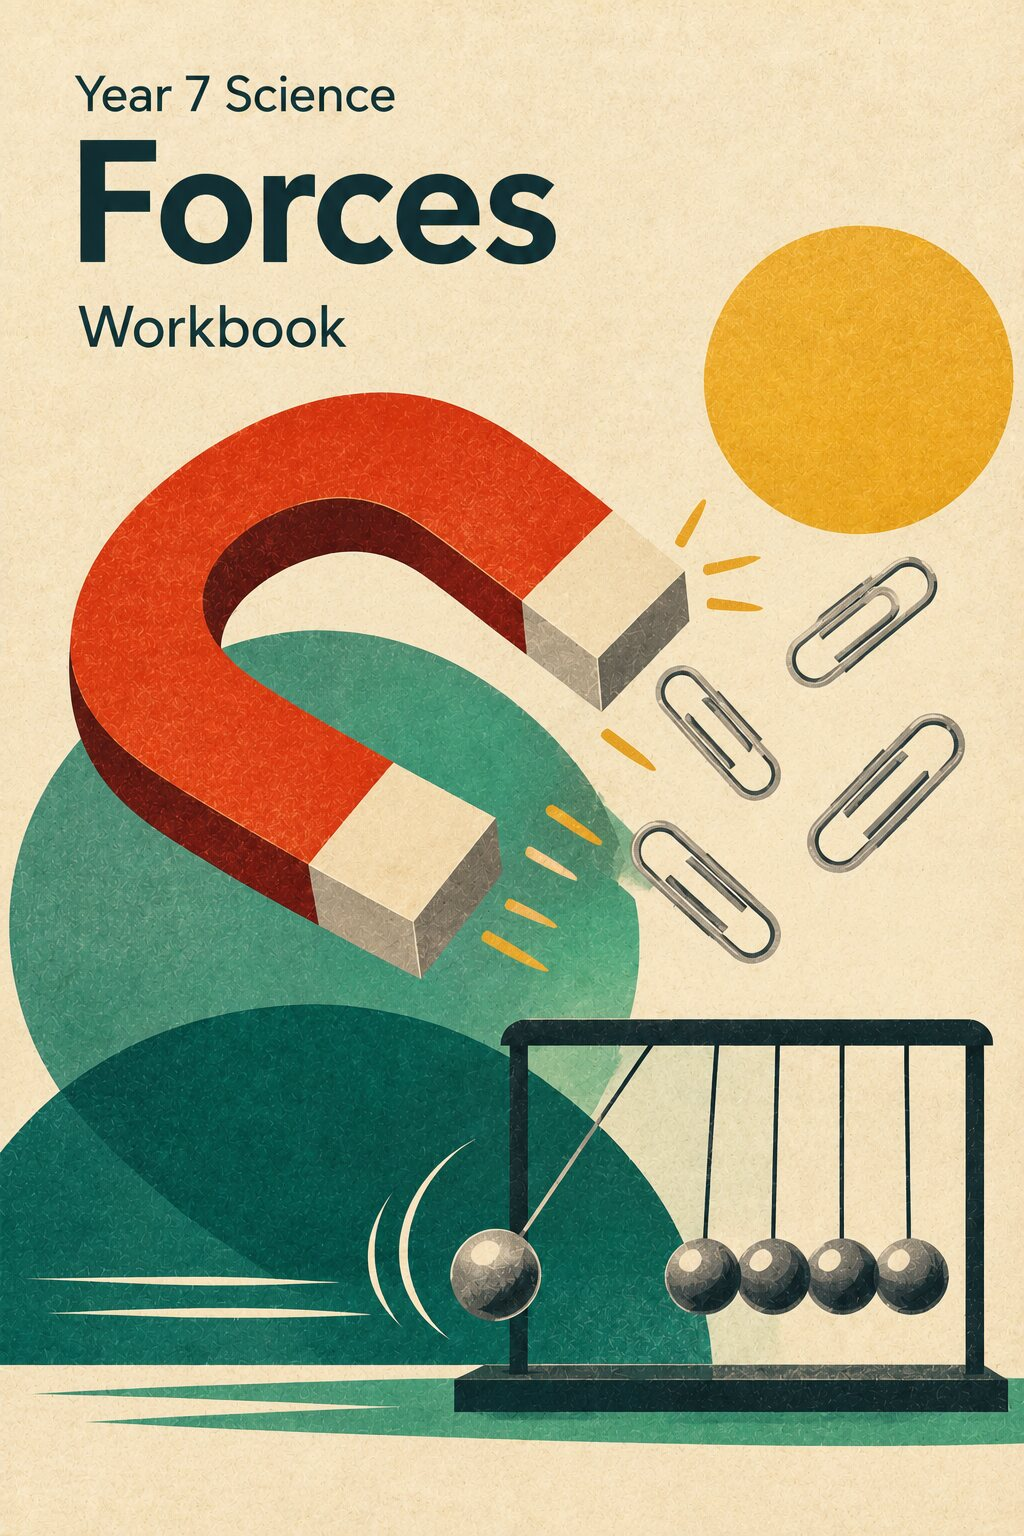
\includegraphics[width=\paperwidth]{../../../covers/forces.jpg}};
  \node[anchor=north east, fill=white, draw=Ink, line width=0.6pt, rounded corners=1.2mm,
        inner xsep=2mm, inner ysep=1.8mm, text width=30mm, font=\headingfont\footnotesize]
    at ([xshift=-4mm, yshift=-4mm]current page.north east)
    {\textbf{Name}\par\vspace{4mm}\hrule\vspace{2mm}\textbf{Class}\par\vspace{4mm}\hrule};
  \node[anchor=south east, fill=white, draw=Ink, line width=0.6pt, rounded corners=1.2mm,
        inner xsep=2.6mm, inner ysep=2mm, font=\headingfont\bfseries, align=right]
    at ([xshift=-4mm, yshift=6mm]current page.south east)
    {Lesson Booklet 3\\[-1pt]{\normalfont\headingfont\scriptsize Lessons 11--14}};
\end{tikzpicture}
\mbox{}
\clearpage

% ---- Inside cover ---------------------------------------------------------
\thispagestyle{plain}
{\headingfont\bfseries\fontsize{22}{26}\selectfont Forces and Motion}\par\vspace{1mm}
{\headingfont\large Lesson Booklet 3 \textbullet\ Lessons 11--14 \textbullet\ Year 7}\par\vspace{1mm}
{\small\itshape VC 2.0: VC2S8U13 \textbullet\ VC2S8U14 \textbullet\ VC2S8U15 \textbullet\ VC2S8I01--I08}\par\vspace{4mm}
\textbf{Teacher}\ \hrulefill\par

\begin{countrybox}{Acknowledgement of Country}
This booklet was created on the unceded Country of the Wurundjeri Woi-wurrung people of the Kulin Nation. We acknowledge Elders past, present and emerging.
\end{countrybox}

\begin{infobox}{How this booklet works}
One section for each lesson. Each opens with its key vocabulary, then:\par\smallskip
\renewcommand{\arraystretch}{1.25}
\begin{tabular}{@{}p{24mm}p{70mm}@{}}
\textbf{Part A} & a reading with comprehension questions \\
\textbf{Part B} & the ideas, worked through \\
\textbf{Part C} & practice on your own \\
\textbf{Part D} & above level: Year 8 extension \\
\end{tabular}

\smallskip
\begin{tabular}{@{}p{24mm}p{70mm}@{}}
\textbf{I do} \tagicon{\icodots{1}} & your teacher works an example (solid frame) \\
\textbf{We do} \tagicon{\icodots{2}} & you try one together (dashed frame) \\
\textbf{Reading} \tagicon{\icoread} & a passage to read (thin frame) \\
\textbf{Above level} \tagicon{\icoup} & extension (double frame) \\
\end{tabular}

\smallskip
Three lesson books. The five experiments are in the \textbf{Experiment Booklet}; the trebuchet investigation has its own booklet.
\end{infobox}

\clearpage
\markboth{Contents}{Contents}
{\headingfont\bfseries\LARGE Contents}\par\vspace{1mm}\noindent\rule{\linewidth}{0.6pt}\par\vspace{2mm}
\renewcommand{\arraystretch}{1.12}
\begin{tabular}{|C{1.1cm}|L{6.0cm}|C{2.4cm}|}
  \hline\thead{Lesson} & \thead{Title} & \thead{Page} \\ \hline
  1 & What is a Force? & Book 1 \\ \hline
  2 & Force Diagrams and Net Force & Book 1 \\ \hline
  3 & \textit{Experiment 1 --- Everyday Forces} & {\footnotesize Experiment Booklet} \\ \hline
  4 & Newton's First and Third Laws & Book 1 \\ \hline
  5 & Newton's Second Law: \texorpdfstring{$F = ma$}{F = ma} & Book 2 \\ \hline
  6 & \textit{Experiment 2 --- Friction and Mass} & {\footnotesize Experiment Booklet} \\ \hline
  7 & Energy and Transformation & Book 2 \\ \hline
  8 & \textit{Experiment 3 --- Bounce Efficiency} & {\footnotesize Experiment Booklet} \\ \hline
  9 & Simple Machines and Levers & Book 2 \\ \hline
  10 & \textit{Experiment 4 --- Lever Mechanical Advantage} & {\footnotesize Experiment Booklet} \\ \hline
  11 & \hyperlink{lesson.11.1}{Levers Extension (Optional)} & \hyperlink{lesson.11.1}{p.\ \pageref{sec:11}} \\ \hline
  12 & \hyperlink{lesson.12.1}{Projectile Motion} & \hyperlink{lesson.12.1}{p.\ \pageref{sec:12}} \\ \hline
  13 & \textit{Experiment 5 --- Measuring $g$} & {\footnotesize Experiment Booklet} \\ \hline
  14 & \hyperlink{lesson.14.1}{Optimising Range (Optional)} & \hyperlink{lesson.14.1}{p.\ \pageref{sec:14}} \\ \hline
  15 & \textit{Trebuchet investigation: planning} & {\footnotesize Trebuchet booklet} \\ \hline
  16 & \textit{Trebuchet investigation: launches} & {\footnotesize Trebuchet booklet} \\ \hline
  17 & \textit{Trebuchet investigation: analysis and conclusion} & {\footnotesize Trebuchet booklet} \\ \hline
  --- & \hyperlink{glossary}{Glossary} & \hyperlink{glossary}{\pageref{sec:glossary}} \\ \hline
\end{tabular}
\renewcommand{\arraystretch}{1}
\clearpage
\setcounter{section}{10}\renewcommand{\lessonart}{11}
% ══════════════════════════════════════════════════════════════════════════════
%  LESSON 11 — LEVERS EXTENSION (OPTIONAL)                          (Week 4 · P2)
% ══════════════════════════════════════════════════════════════════════════════
\sectiondiv{Levers Extension (Optional)}{Year 8 extension \textbullet{} Turning effects \textbullet{} Arcs and tip speed \textbullet{} Energy and launch speed}\label{sec:11}
\lessoncodes{VC2S8U13 \textbullet{} VC2S8U15 \textbullet{} VC2S10U15 (above level)}

\vocabhead
\begin{ctab}
\begin{tabular}{|SW{2.91cm}|W{8.05cm}|}
  \hd & \thead{Word} & \thead{Definition (copy from the slide)} \\ \hline
  & \scaf{\textbf{Turning effect}\label{voc:turning-effect}} & \scaf{How strongly a force turns something about a pivot: force $\times$ distance from the pivot.} \\ \hline
  & \textbf{Counterweight}\label{voc:counterweight} & \cell{11.v2} \\ \hline
  & \textbf{Arc}\label{voc:arc} & \cell{11.v3} \\ \hline
  & \textbf{Tip speed}\label{voc:tip-speed} & \cell{11.v4} \\ \hline
  & \textbf{Launch speed}\label{voc:launch-speed} & \cell{11.v5} \\ \hline
\end{tabular}
\end{ctab}

\optionalnote{Every part of this lesson goes beyond the Year 7 standard. Your teacher may skip it --- Lesson~12 follows straight on from Lesson~10.}

% ─── PART A ───────────────────────────────────────────────────────────────────
\lessonpart{A}{Reading and comprehension}{Teal}\label{read:11}

\begin{readingbox}{Reading --- Warwolf, the Biggest Trebuchet}
\small % one size down so the whole reading fits on the lesson's first page
In 1304 King Edward I of England laid siege to Stirling Castle in Scotland. For weeks his siege engines battered the walls. To finish the job, Edward ordered his chief engineer, Master James of St George, to build something far bigger: a trebuchet called \emph{Warwolf}. It is believed to be the largest trebuchet ever made. Records say it took five master carpenters and forty-nine other labourers at least three months to build, and when it was taken apart it filled thirty wagons.

A trebuchet is a giant Class 1 lever. A heavy counterweight hangs from the short arm. When it is released it falls, and the long arm swings up and over, flinging a stone from a sling at its end. The counterweight only drops a few metres, but in the same moment the tip of the long arm sweeps through a huge arc --- so the tip moves far faster than the counterweight.

The energy for the throw comes from the falling counterweight. Its gravitational potential energy becomes kinetic energy of the arm, the sling and the stone. The arms decide how that energy is shared out. A longer throwing arm moves its tip faster, but no arrangement of arms can give the stone more energy than the counterweight loses --- and some is always wasted.

The castle's small garrison, only about thirty men, offered to surrender before Warwolf was ready. Edward refused to accept until he had seen his new machine work. One medieval chronicle claims that a single stone from Warwolf smashed through two of the castle's walls.
\end{readingbox}

\rcreset
\rcqk{11.c1}{Who ordered Warwolf to be built, and where and when was it used?}{1.5cm}
\rcqk{11.c2}{Explain why a trebuchet is a Class 1 lever. Name its effort and its load.}{1.7cm}
\rcqk{11.c3}{The counterweight only drops a few metres. Explain why the tip of the long arm moves so much faster than the counterweight.}{1.9cm}
\rcqk{11.c4}{Where does the energy for the throw come from? Describe the energy transformation.}{1.7cm}
\rcqk{11.c5}{Which phrase in the third paragraph tells you that a lever cannot create energy?}{1.4cm}
\rcqk{11.c6}{Give two pieces of evidence from the passage that show how big Warwolf was.}{1.5cm}
\rcqk{11.c7}{Suggest why Edward refused to accept the surrender until Warwolf had been tested.}{1.7cm}
\rcqk{11.c8}{Suppose Warwolf's counterweight had been made heavier, with the arms kept the same. Using the passage, predict what would happen to the energy available and to the speed of the stone, and explain why.}{2.0cm}

% ─── PART B ───────────────────────────────────────────────────────────────────
\lessonpart{B}{Theory and examples}{Blue}\label{theory:11}

\subsection{Turning Effects}\label{sub:11.1}

A force that acts on a lever tries to turn it about the pivot. Its \textbf{turning effect} (also called its \emph{moment}) depends on the size of the force and how far from the pivot it acts.

\begin{infobox}{Turning effect}
\[ \text{turning effect} = \text{force} \times \text{distance from the pivot} \]
Force in newtons (N), distance in metres (m), turning effect in \textbf{newton metres (N\,m)}.\\[3pt]
A lever balances when the total turning effect one way equals the total turning effect the other way. With two or more loads on one side, \textbf{add} their turning effects.
\end{infobox}

The law of the lever from Lesson~9 is a special case: effort $\times$ effort arm and load $\times$ load arm are the two turning effects.

\begin{workedex}{Two children on one side}
On one side of a seesaw, a 300\,N child sits 2.0\,m from the pivot and a 200\,N child sits 1.0\,m from the pivot. Where must a 400\,N child sit on the other side to balance it?

\medskip
\textbf{Left side:}\quad $300 \times 2.0 + 200 \times 1.0 = 600 + 200 = 800$\,N\,m

\textbf{Right side:}\quad $400 \times d = 800$ \quad so \quad $d = 800 \div 400 = \mathbf{2.0\ \text{m}}$
\end{workedex}
\begin{wedo}{Two children on one side}
On one side of a seesaw, a 200\,N child sits 1.5\,m from the pivot and a 300\,N child sits 0.5\,m from the pivot. Where must a 450\,N adult sit on the other side to balance it?
\wbox{11.wd1}{3.0cm}
\end{wedo}
\newpage
\subsection{Arcs and Tip Speed}\label{sub:11.2}

When a lever arm turns, every point on it turns through the \textbf{same angle in the same time}. A point far from the pivot travels around a bigger circle, so it covers a longer arc --- and moves faster.

\diagArmArcs
\figcap[fig:arm-arcs]{Both ends of the arm turn through the same angle in the same time, but the end of the long arm travels a much longer arc.}

\begin{infobox}{Arc length and speed}
\[ \text{arc length} = \frac{\text{angle}}{360} \times 2 \times \pi \times r \qquad\qquad \text{average speed} = \frac{\text{arc length}}{\text{time}} \]
$r$ = distance from the pivot (m) \quad Use $\pi \approx 3.14$.\\[3pt]
For two points on the same arm: \quad $\dfrac{\text{tip speed}}{\text{counterweight speed}} = \dfrac{\text{long arm}}{\text{short arm}}$
\end{infobox}

\begin{workedex}{Speed of the arm tip}
A trebuchet's long arm is 2.0\,m long. During a launch it sweeps through 90$^\circ$ in 0.25\,s. Find the arc travelled by the tip, and the tip's average speed.

\medskip
\textbf{Arc:}\quad $\tfrac{90}{360} \times 2 \times 3.14 \times 2.0 = 0.25 \times 12.56 = 3.14$\,m

\textbf{Speed:}\quad $3.14 \div 0.25 = \mathbf{12.6\ \text{m/s}}$
\end{workedex}

\begin{wedo}{Speed of the arm tip}
A model trebuchet's long arm is 1.5\,m long. During a launch it sweeps through 90$^\circ$ in 0.3\,s. Use $\pi = 3.14$.
\pt{a}Find the arc travelled by the tip.
\wbox{11.wd2a}{1.8cm}
\pt{b}Find the tip's average speed.
\wbox{11.wd2b}{1.6cm}
\end{wedo}

\begin{workedex}{Speed of the counterweight end}
The same trebuchet has a short arm of 0.4\,m. How fast does the counterweight end of the arm move?

\medskip
\textbf{Ratio:}\quad long arm $\div$ short arm $= 2.0 \div 0.4 = 5$, so the tip moves 5 times as fast.

\textbf{Speed:}\quad $12.6 \div 5 \approx \mathbf{2.5\ \text{m/s}}$
\end{workedex}

\begin{wedo}{Speed of the counterweight end}
The same model trebuchet has a short arm of 0.5\,m, and its tip moves at about 7.9\,m/s. How fast does the counterweight end of the arm move?
\wbox{11.wd3}{2.4cm}
\end{wedo}

\subsection{Energy Sets the Limit}\label{sub:11.3}

The arms share out the speed, but the energy comes from the falling counterweight. The stone's kinetic energy can never be more than the gravitational potential energy the counterweight gives up --- and because some energy is always wasted, it is always less.

\begin{infobox}{From counterweight to launch speed}
$\text{GPE lost} = m \times g \times h$ \quad(counterweight mass and drop)\\[2pt]
$\text{KE of stone} = \text{efficiency} \times \text{GPE lost}$\\[2pt]
$\text{KE} = \tfrac{1}{2}mv^2 \quad\Rightarrow\quad v = \sqrt{2 \times \text{KE} \div m}$ \quad(stone mass)
\end{infobox}

\begin{workedex}{Launch speed from energy}
A 20\,kg counterweight falls 0.8\,m. The trebuchet is 25\% efficient and the stone has a mass of 0.2\,kg. Find the stone's launch speed. Use $g = 9.8$\,N/kg.

\medskip
\textbf{GPE lost:}\quad $20 \times 9.8 \times 0.8 = 156.8$\,J

\textbf{KE of stone:}\quad $0.25 \times 156.8 = 39.2$\,J

\textbf{Speed:}\quad $v^2 = 2 \times 39.2 \div 0.2 = 392$, \quad so \quad $v = \sqrt{392} \approx \mathbf{19.8\ \text{m/s}}$
\end{workedex}
\begin{wedo}{Launch speed from energy}
An 8\,kg counterweight falls 1.0\,m. The trebuchet is 25\% efficient and the stone has a mass of 0.2\,kg. Use $g = 9.8$\,N/kg.
\pt{a}Find the GPE the counterweight gives up.
\wbox{11.wd4a}{1.6cm}
\pt{b}Find the kinetic energy of the stone and its launch velocity.
\wbox{11.wd4b}{1.6cm}
\end{wedo}

% ─── PART C ───────────────────────────────────────────────────────────────────
\lessonpart{C}{Practice}{Amber}\label{prac:11}

Every question in this lesson goes beyond the Year 7 standard. Use $g = 9.8$\,N/kg and $\pi \approx 3.14$. Show your working, and always include the unit.

\taskpair{A 40\,N force pushes on a door 0.5\,m from its hinges. Find its turning effect.}{\wbox{11.t1}{2.4cm}}
         {Which has the bigger turning effect: 60\,N acting 0.4\,m from a pivot, or 30\,N acting 0.9\,m from it? Show your working.}{\wbox{11.t2}{2.4cm}}

\needspace{10\baselineskip}
\task A mechanic pushes on a spanner with 50\,N, 0.25\,m from the nut.
\pt{a}Find the turning effect.
\wbox{11.t3a}{2.0cm}
\pt{b}What force would give the same turning effect if she pushed only 0.10\,m from the nut?
\wbox{11.t3b}{2.0cm}

\needspace{10\baselineskip}
\task On one side of a seesaw, a 250\,N child sits 1.6\,m from the pivot and a 150\,N child sits 1.0\,m from the pivot. Where must a 500\,N adult sit on the other side to balance it?
\wbox{11.t4}{2.8cm}

\needspace{12\baselineskip}
\task Complete the table. Use arc length $= \tfrac{\text{angle}}{360} \times 2 \times \pi \times r$.

\vspace{4pt}
\begin{ctab}
\begin{tabular}{|SZ{2.71cm}|Z{2.71cm}|Z{5.11cm}|}
  \hd & \thead{Angle turned} & \thead{Distance from pivot $r$ (m)} & \thead{Arc length (m)} \\ \hline
  & 90$^\circ$  & 2.0 & \scaf{$\tfrac{90}{360} \times 2 \times 3.14 \times 2.0 = 3.14$} \\ \hline
  & 90$^\circ$  & 1.0 & \cell{11.t5-r2c3} \\ \hline
  & 180$^\circ$ & 2.0 & \cell{11.t5-r3c3} \\ \hline
  & 60$^\circ$  & 1.2 & \cell{11.t5-r4c3} \\ \hline
\end{tabular}
\end{ctab}

\taskpair{The tip of a trebuchet arm sweeps along a 4.8\,m arc in 0.3\,s. Find its average speed.}{\wbox{11.t6}{2.4cm}}
         {A trebuchet has a long arm of 3.0\,m and a short arm of 0.6\,m. The counterweight end moves at 3\,m/s. How fast does the tip move?}{\wbox{11.t7}{2.4cm}}

\needspace{10\baselineskip}
\task Two trebuchets both have a short arm of 0.5\,m. Trebuchet A has a long arm of 2.0\,m; trebuchet B has a long arm of 3.0\,m. In both, the counterweight end moves at 2.4\,m/s.
\pt{a}Find the tip speed of each trebuchet.
\wbox{11.t8a}{2.0cm}
\pt{b}Which one launches its stone faster, and why?
\abox{11.t8b}{2.0cm}

\taskpair{A 15\,kg counterweight falls 1.0\,m. Find the GPE it gives up.}{\wbox{11.t9}{2.4cm}}
         {A 0.1\,kg stone leaves a trebuchet at 18\,m/s. Find its kinetic energy.}{\wbox{11.t10}{2.4cm}}

\needspace{10\baselineskip}
\task A counterweight gives up 150\,J of GPE, and the stone gains 45\,J of kinetic energy. Find the efficiency of the trebuchet, and name two places the rest of the energy went.
\wbox{11.t11}{2.8cm}

\needspace{10\baselineskip}
\task A 12\,kg counterweight falls 1.5\,m. The trebuchet is 25\% efficient, and the stone has a mass of 0.15\,kg.
\pt{a}Find the GPE the counterweight gives up.
\wbox{11.t12a}{2.0cm}
\pt{b}Find the KE given to the stone.
\wbox{11.t12b}{2.0cm}
\pt{c}Find the stone's launch speed.
\wbox{11.t12c}{2.0cm}

\needspace{10\baselineskip}
\task Explain, in your own words, why making the long arm longer makes the tip move faster, but cannot make the stone go faster and faster without any limit.
\abox{11.t13}{2.8cm}

% ─── PART D ───────────────────────────────────────────────────────────────────
\lessonpart{D}{Challenge}{Violet}\label{ext:11}

\begin{yr8box}
The hardest questions in this extension lesson. They ask you to check a claim, combine turning effects with energy, or design a better trebuchet.

\medskip
\needspace{10\baselineskip}
\exttask Sam says his model trebuchet, with a 2\,kg counterweight that falls 0.5\,m, launched a 0.05\,kg ball at 25\,m/s. Use energy to decide whether this is possible. Show your working.
\wbox{11.x14}{3.0cm}

\needspace{10\baselineskip}
\exttask A trebuchet has a short arm of 0.4\,m. The builders want the tip to move 6 times as fast as the counterweight end.
\pt{a}How long must the long arm be?
\wbox{11.x15a}{2.0cm}
\pt{b}Suggest one practical problem with making the long arm very long.
\abox{11.x15b}{2.0cm}

\needspace{10\baselineskip}
\exttask Before launch, a trebuchet arm is held level. A 30\,kg counterweight hangs 0.5\,m from the pivot on the short side. The arm's own weight, 100\,N, acts 0.6\,m from the pivot on the long side. A trigger rope pulls straight down on the end of the long arm, 2.5\,m from the pivot. Find the force in the trigger rope.
\wbox{11.x16}{3.4cm}

\needspace{10\baselineskip}
\exttask During a launch, a trebuchet arm turns through 120$^\circ$ in 0.4\,s. Its long arm is 2.4\,m and its short arm is 0.6\,m.
\pt{a}Find the arc travelled by the tip, and its average speed.
\wbox{11.x17a}{2.0cm}
\pt{b}Find the average speed of the counterweight end.
\wbox{11.x17b}{2.0cm}
\pt{c}Check that your two speeds are in the same ratio as the arm lengths.
\wbox{11.x17c}{2.0cm}

\needspace{10\baselineskip}
\exttask A 25\,kg counterweight falls 1.2\,m, and launches a 0.2\,kg stone at 15\,m/s.
\pt{a}Calculate the efficiency of this trebuchet.
\wbox{11.x18a}{2.0cm}
\pt{b}Most of the energy did not reach the stone. Suggest where it went --- think about what is still moving when the stone leaves the sling.
\abox{11.x18b}{2.0cm}

\needspace{18\baselineskip}
\exttask A counterweight gives up 200\,J. The stone gets 60\,J, the counterweight and arm are still moving with 90\,J, and 50\,J becomes thermal energy and sound. Draw a Sankey diagram using a scale of \textbf{1\,cm = 20\,J}. Label each arrow with its energy.

\vspace{3pt}
\drawk{11.x19}{4.6cm}{
\textit{\color{MidGrey}Draw your Sankey diagram here: energy in on the left, the useful energy straight on, the other energy turning down.}
}

\needspace{10\baselineskip}
\exttask Real trebuchets fling the stone from a sling that hangs from the end of the long arm. Use the idea of arcs and tip speed to explain how the sling helps the stone leave faster.
\abox{11.x20}{3.0cm}
\end{yr8box}

\newpage
\setcounter{section}{11}\renewcommand{\lessonart}{12}
% ══════════════════════════════════════════════════════════════════════════════
%  LESSON 12 — PROJECTILE MOTION                                     (Week 4 · P3)
% ══════════════════════════════════════════════════════════════════════════════
\sectiondiv{Projectile Motion}{Projectiles \textbullet{} Two independent motions \textbullet{} Time of flight \textbullet{} Measuring $g$}\label{sec:12}
\lessoncodes{VC2S8U14 \textbullet{} VC2S8H01 \textbullet{} VC2S10U17 (above level)}

\vocabhead
\begin{ctab}
\begin{tabular}{|SW{2.91cm}|W{8.05cm}|}
  \hd & \thead{Word} & \thead{Definition (copy from the slide)} \\ \hline
  & \scaf{\textbf{Projectile}\label{voc:projectile}} & \scaf{An object that is thrown or launched and then moves under gravity alone.} \\ \hline
  & \textbf{Trajectory}\label{voc:trajectory} & \cell{12.v2} \\ \hline
  & \textbf{Horizontal}\label{voc:horizontal} & \cell{12.v3} \\ \hline
  & \textbf{Vertical}\label{voc:vertical} & \cell{12.v4} \\ \hline
  & \textbf{Independent motions}\label{voc:independent-motions} & \cell{12.v5} \\ \hline
  & \textbf{Time of flight}\label{voc:time-of-flight} & \cell{12.v6} \\ \hline
\end{tabular}
\end{ctab}

% ─── PART A ───────────────────────────────────────────────────────────────────
\lessonpart{A}{Reading and comprehension}{Teal}\label{read:12}

\begin{readingbox}{Reading --- Galileo and the Two Motions}
\small % one size down so the whole reading fits on the lesson's first page
How does a cannonball fly? In 1537 the Italian mathematician Niccolò Tartaglia published one of the first books to use mathematics to study gunnery. He described a cannonball leaving the barrel in a straight line, then curving around in an arc, and finally dropping straight down to the ground. Gunnery books repeated his ideas for many years.

About a hundred years later, Galileo Galilei worked out what really happens, and he published it in 1638. He realised that a projectile is doing \emph{two things at once}, and that the two motions do not affect each other. Sideways, once the ball is launched nothing pushes or pulls it (if we ignore the air), so it keeps moving sideways at a steady speed. Downwards, gravity pulls it, so it speeds up as it falls --- exactly as if it had simply been dropped. Put a steady sideways motion together with a speeding-up downwards motion and you get a smooth curve called a \emph{parabola}, with no straight sections at all.

The result that surprises people most is this. Launch one ball sideways and drop an identical ball from the same height at the same moment: they hit the ground at the same time. The launched ball lands far away, but its sideways speed makes no difference to how quickly gravity pulls it down.

That is why a launched ball and a dropped ball speed up downwards at exactly the same rate --- a rate you will measure in Experiment~5. Galileo's idea replaced a model that had been trusted for a century --- a good example of science changing when someone finds better evidence and better reasoning.
\end{readingbox}

\rcreset
\rcqk{12.c1}{Describe the path Tartaglia thought a cannonball followed.}{1.5cm}
\rcqk{12.c2}{Galileo said a projectile does ``two things at once''. Describe each motion.}{1.8cm}
\rcqk{12.c3}{According to the passage, why does a projectile's sideways speed stay the same?}{1.5cm}
\rcqk{12.c4}{What is the name of the curved path that Galileo described?}{1.2cm}
\rcqk{12.c5}{Explain why a ball launched sideways and a ball dropped from the same height land at the same time.}{1.9cm}
\rcqk{12.c6}{Which phrase in the second paragraph tells you that the sideways motion and the downwards motion are independent?}{1.4cm}
\rcqk{12.c7}{How does the passage show that scientific ideas can change? Give the old idea and the new one.}{1.8cm}

% ─── PART B ───────────────────────────────────────────────────────────────────
\lessonpart{B}{Theory and examples}{Blue}\label{theory:12}

\subsection{What is a Projectile?}\label{sub:12.1}

A \textbf{projectile} is an object that has been launched and is then moving with only gravity acting on it. A thrown ball, water from a drinking fountain and a stone flung by a trebuchet are all projectiles. (We ignore air resistance, which is small for heavy, slow objects.) The curved path of a projectile is called its \textbf{trajectory}.

\diagProjectile
\figcap[fig:projectile]{A ball launched sideways from height $h$ lands a horizontal distance $R$ away. Once launched, the only force on it is its weight, $W$.}

\subsection{Two Independent Motions}\label{sub:12.2}

\vspace{2pt}
\begin{ctab}
\begin{tabular}{|L{2.20cm}|L{3.95cm}|L{4.39cm}|}
  \thead{} & \thead{Sideways (horizontal)} & \thead{Downwards (vertical)} \\ \hline
  Force acting & none (ignoring air) & gravity (the ball's weight) \\ \hline
  Speed        & stays the same       & increases by 9.8\,m/s every second \\ \hline
  Distance     & the same in every second & more in every second \\ \hline
\end{tabular}
\end{ctab}

\diagTwoMotions
\figcap[fig:two-motions]{Positions every 0.1\,s. At every moment the launched ball is at the same height as the dropped ball, so they land together. Sideways, the launched ball moves the same distance in each 0.1\,s.}

\subsection{Time of Flight}\label{sub:12.3}

The time a projectile spends in the air depends only on the height it falls from, not on its sideways speed.

\begin{infobox}{Key equations --- launched sideways}
\[
  h = \tfrac{1}{2}g t^2
  \quad\Rightarrow\quad
  t = \sqrt{\frac{2h}{g}}
  \qquad\qquad
  R = v \times t
  \qquad\qquad
  g = \frac{2h}{t^2}
\]
$h$ = drop height (m) \quad $t$ = time of flight (s) \quad $g = 9.8$\,m/s$^2$\\
$v$ = sideways launch speed (m/s) \quad $R$ = range (m)
\end{infobox}

\begin{workedex}{Time of flight}
A ball rolls off a table 1.25\,m high. How long does it take to land?

\medskip
\textbf{Step 1:}\quad $2h = 2 \times 1.25 = 2.5$

\textbf{Step 2:}\quad $2.5 \div 9.8 = 0.255$

\textbf{Step 3:}\quad $t = \sqrt{0.255} \approx \mathbf{0.51\ \text{s}}$
\end{workedex}

\begin{wedo}{Time of flight}
A ball rolls off a table 0.60\,m high. Use $t = \sqrt{2h \div 9.8}$ to find how long it takes to land.
\wbox{12.wd1}{2.8cm}
\end{wedo}

\subsection{How Far Does It Go?}\label{sub:12.4}

While the ball falls, it keeps moving sideways at its launch speed. So the distance it travels sideways is its launch speed multiplied by its time in the air.

\begin{workedex}{Range}
The ball in Worked Example~\ref{we:12.1} leaves the table at 3.0\,m/s. How far from the table does it land?

\medskip
$R = v \times t = 3.0 \times 0.51 \approx \mathbf{1.5\ \text{m}}$
\end{workedex}

\begin{wedo}{Range}
A ball rolls off a table 0.60\,m high at 2.5\,m/s, and is in the air for 0.35\,s. How far from the table does it land?
\wbox{12.wd2}{2.4cm}
\end{wedo}

\subsection{Measuring $g$}\label{sub:12.5}

The table in Section~\ref{sub:12.2} says that a falling object's speed goes up by 9.8\,m/s every second. That number is $g$. You could find it from a drop height and a fall time, using $g = 2h \div t^2$ from the key equations box. Experiment~5 measures it more directly, by watching a falling object speed up. A \textbf{motion sensor} above the object measures how fast it is moving 50 times every second, and draws a \textbf{velocity--time graph}. (Velocity is speed in one direction --- here, downwards.) While the object falls, the line on the graph is straight and slopes up, because its speed goes up by the same amount every second.

\diagVelocityTime{numbers}
\figcap[fig:velocity-time]{A velocity--time graph for a ball dropped under a motion sensor. The ball is held still, let go at 0.10\,s, and lands at 0.55\,s.}

\begin{infobox}{Acceleration from a velocity--time graph}
\textbf{Time of fall} $=$ time it lands $-$ time it is let go\\[2pt]
\textbf{Change in speed} $=$ final velocity $-$ starting velocity\\[2pt]
\textbf{Acceleration} $=$ change in speed $\div$ time of fall \qquad (for a falling object, this is $g$)
\end{infobox}

\begin{workedex}{Finding $g$ from a velocity--time graph}
Use the graph in Figure~\ref{fig:velocity-time} to find the ball's acceleration.

\medskip
\textbf{Read the graph:}\quad starting velocity $= 0$\,m/s, \quad final velocity $= 4.4$\,m/s

\textbf{Time of fall:}\quad $0.55 - 0.10 = 0.45$\,s

\textbf{Change in speed:}\quad $4.4 - 0 = 4.4$\,m/s

\textbf{Acceleration:}\quad $4.4 \div 0.45 \approx \mathbf{9.8\ \text{m/s}^2}$ \quad --- the accepted value of $g$.
\end{workedex}

\begin{wedo}{Finding $g$ from a velocity--time graph}
A motion sensor's graph for a falling tennis ball shows a starting velocity of 0.2\,m/s and a final velocity of 3.1\,m/s. The fall took 0.30\,s.
\ptpair{a}{Find the change in speed.}{\wbox{12.wd3a}{1.8cm}}{b}{Find the acceleration.}{\wbox{12.wd3b}{1.8cm}}
\end{wedo}

% ─── PART C ───────────────────────────────────────────────────────────────────
\lessonpart{C}{Practice}{Amber}\label{prac:12}

Work through every task. Use $g = 9.8$\,m/s$^2$ and ignore air resistance. Show your working, and always include the unit.

\needspace{12\baselineskip}
\task Is each object a projectile? Write \textbf{YES} or \textbf{NO} in the box.

\vspace{4pt}
\begin{ctab}
\begin{tabular}{|SW{3.69cm}|Z{1.37cm}|W{3.69cm}|Z{1.37cm}|}
  \hd & \thead{Object} & \thead{\scriptsize Projectile?} & \thead{Object} & \thead{\scriptsize Projectile?} \\ \hline
  & A basketball after it leaves the player's hands & \scaf{YES} & A rocket with its engine on & \scaf{NO} \\ \hline
  & A stone flying from a trebuchet & \cell{12.t1-r2c2} & A car driving along a road & \cell{12.t1-r2c4} \\ \hline
  & Water arcing from a drinking fountain & \cell{12.t1-r3c2} & A ball rolling off the edge of a table & \cell{12.t1-r3c4} \\ \hline
\end{tabular}
\end{ctab}

\needspace{12\baselineskip}
\task Complete the table for a ball that has been launched sideways.

\vspace{4pt}
\begin{ctab}
\begin{tabular}{|SW{3.13cm}|W{3.70cm}|W{3.70cm}|}
  \hd & \thead{} & \thead{Sideways motion} & \thead{Downwards motion} \\ \hline
  & What force acts? & \scaf{none (ignoring air)} & \cell{12.t2-r1c3} \\ \hline
  & What happens to the speed? & \cell{12.t2-r2c2} & \cell{12.t2-r2c3} \\ \hline
\end{tabular}
\end{ctab}

\needspace{10\baselineskip}
\task One ball is dropped, and an identical ball is launched sideways from the same height at the same moment. The dropped ball lands after 0.6\,s. When does the launched ball land? Explain.
\abox{12.t3}{2.4cm}

\taskpair{A ball rolls off a table 0.80\,m high. Find its time of flight.}{\wbox{12.t4}{2.4cm}}
         {A ball rolls off a ledge 2.0\,m high. Find its time of flight.}{\wbox{12.t5}{2.4cm}}

\taskpair{A ball is launched sideways at 4.0\,m/s and is in the air for 0.50\,s. How far does it travel sideways?}{\wbox{12.t6}{2.4cm}}
         {A ball launched sideways lands 2.4\,m away after 0.60\,s. Find its launch speed.}{\wbox{12.t7}{2.4cm}}

\taskpair{A ball falls 2.0\,m in 0.64\,s. Calculate $g$.}{\wbox{12.t8}{2.4cm}}
         {A motion sensor shows a falling ball speed up from 1.0\,m/s to 4.0\,m/s in 0.31\,s. Find its acceleration.}{\wbox{12.t9}{2.4cm}}

\needspace{10\baselineskip}
\task A marble rolls off a desk 0.45\,m high at 2.0\,m/s.
\pt{a}Find its time of flight.
\wbox{12.t10a}{2.0cm}
\pt{b}Find how far from the desk it lands.
\wbox{12.t10b}{2.0cm}

\needspace{10\baselineskip}
\task A group measures $g = 9.2$\,m/s$^2$. Calculate their percentage error, using
\[ \% \text{ error} = \frac{|\text{measured } g - 9.8|}{9.8} \times 100\% \]
\wbox{12.t11}{2.6cm}

\needspace{10\baselineskip}
\task Two marbles roll off the same desk at the same moment, one at 1\,m/s and one at 3\,m/s.
\pt{a}Which one lands first?
\abox{12.t12a}{2.0cm}
\pt{b}Which one lands further from the desk?
\abox{12.t12b}{2.0cm}
\pt{c}Explain both answers using the idea of two independent motions.
\abox{12.t12c}{2.0cm}

\needspace{10\baselineskip}
\task Priya says: \emph{``The faster I roll a ball off the table, the longer it stays in the air.''} Is Priya right? Explain.
\abox{12.t13}{2.6cm}

% ─── PART D ───────────────────────────────────────────────────────────────────
\lessonpart{D}{Above level}{Violet}\label{ext:12}

\begin{yr8box}
These questions go beyond the Year 7 standard. They ask you to combine equations, compare situations, or evaluate a method.

\medskip
\needspace{10\baselineskip}
\exttask On the Moon, $g = 1.6$\,m/s$^2$. A ball rolls off a 1.25\,m ledge at 2.0\,m/s.
\pt{a}Find its time of flight and how far it travels sideways.
\wbox{12.x14a}{2.0cm}
\pt{b}Compare your answers with the same roll on Earth ($t = 0.51$\,s). Explain the difference.
\abox{12.x14b}{2.0cm}

\needspace{10\baselineskip}
\exttask Ball A rolls off a 0.45\,m step and ball B rolls off a 1.80\,m wall.
\pt{a}Find the time of flight of each ball.
\wbox{12.x15a}{2.0cm}
\pt{b}B fell four times as far as A. How many times as long did it take? Use $h = \tfrac{1}{2}gt^2$ to explain why.
\wbox{12.x15b}{2.0cm}

\needspace{10\baselineskip}
\exttask A ball rolls off a bench and takes 0.45\,s to land. Use $h = \tfrac{1}{2}gt^2$ to find the height of the bench.
\wbox{12.x16}{2.6cm}

\needspace{10\baselineskip}
\exttask A ball machine fires tennis balls sideways from a height of 1.5\,m at 20\,m/s. Ignoring air resistance, how far do the balls travel before they land?
\wbox{12.x17}{2.8cm}

\needspace{10\baselineskip}
\exttask A group rolls a ball off a 0.80\,m bench and measures a mean value of $g = 10.6$\,m/s$^2$.
\pt{a}Calculate their percentage error.
\wbox{12.x18a}{2.0cm}
\pt{b}Suggest two sources of error in the method, and how each could be reduced.
\abox{12.x18b}{2.0cm}

\needspace{10\baselineskip}
\exttask On a velocity--time graph, the acceleration is the slope (steepness) of the line. A falling ball's line passes through the points (0.10\,s, 1.2\,m/s) and (0.40\,s, 4.1\,m/s).
\pt{a}Find the slope of the line: the change in velocity divided by the change in time.
\wbox{12.x19a}{2.0cm}
\pt{b}Describe how the line would look for the same ball dropped on the Moon, where $g = 1.6$\,m/s$^2$.
\abox{12.x19b}{2.0cm}

\needspace{12\baselineskip}
\exttask Galileo's idea says that sideways speed does not change how long a projectile takes to fall. Design a fair test, using a ramp, a table and a slow-motion video, to check this.
\pt{a}Name the independent and dependent variables.
\abox{12.x20a}{2.0cm}
\pt{b}Name two variables you would keep the same.
\abox{12.x20b}{2.0cm}
\pt{c}Predict what you would find, and give a reason.
\abox{12.x20c}{2.0cm}
\end{yr8box}

\newpage
\setcounter{section}{13}\renewcommand{\lessonart}{14}
% ══════════════════════════════════════════════════════════════════════════════
%  LESSON 14 — OPTIMISING RANGE (OPTIONAL, YEAR 8)                   (Week 5 · P2)
% ══════════════════════════════════════════════════════════════════════════════
\sectiondiv{Optimising Range (Optional)}{Year 8 extension \textbullet{} Launching at an angle \textbullet{} The best angle \textbullet{} Real launches}\label{sec:14}
\lessoncodes{VC2S8U14 \textbullet{} VC2S10U17 (above level)}

\vocabhead
\begin{ctab}
\begin{tabular}{|SW{2.91cm}|W{8.05cm}|}
  \hd & \thead{Word} & \thead{Definition (copy from the slide)} \\ \hline
  & \scaf{\textbf{Launch angle}\label{voc:launch-angle}} & \scaf{The angle between the ground and the direction a projectile is launched in.} \\ \hline
  & \textbf{Range}\label{voc:range} & \cell{14.v2} \\ \hline
  & \textbf{Maximum range}\label{voc:maximum-range} & \cell{14.v3} \\ \hline
  & \textbf{Complementary angles}\label{voc:complementary-angles} & \cell{14.v4} \\ \hline
  & \textbf{Launch height}\label{voc:launch-height} & \cell{14.v5} \\ \hline
\end{tabular}
\end{ctab}

% ─── PART A ───────────────────────────────────────────────────────────────────
\lessonpart{A}{Reading and comprehension}{Teal}\label{read:14}

\begin{readingbox}{Reading --- Why Long Jumpers Don't Take Off at 45$^\circ$}
Ask a physics student how to throw something as far as possible and they will probably say ``at 45 degrees''. On flat ground, with no air, they are right: a ball launched at 45$^\circ$ goes further than at any other angle with the same speed. Launch it flatter and it hits the ground too soon. Launch it steeper and it spends its speed going up instead of along.

So why do the world's best long jumpers take off at only about 20$^\circ$? Because a jumper's speed is not the same at every angle. A sprinter can run at more than 10\,m/s, but nobody can spring \emph{upwards} that fast. To leave the board at 45$^\circ$, a jumper would have to slow right down. A flatter take-off keeps almost all the speed of the run-up, and that matters more than the angle.

Shot-putters also launch lower than 45$^\circ$, at about 35--40$^\circ$. They release the shot from above head height, so it has further to fall, and they can push harder at a flatter angle.

Medieval engineers had to solve the same problem with trebuchets. The stone leaves the sling high above the ground, and air resistance slows it the whole way. The best release angle for a real trebuchet is usually a little below 45$^\circ$ --- and the only way to find it is to test.
\end{readingbox}

\rcreset
\rcqk{14.c1}{On flat ground with no air, what launch angle gives the longest range?}{1.2cm}
\rcqk{14.c2}{Explain why a launch that is too flat, or too steep, does not go as far.}{1.6cm}
\rcqk{14.c3}{Why do long jumpers take off at about 20$^\circ$ instead of 45$^\circ$?}{1.6cm}
\rcqk{14.c4}{Give two reasons why a real trebuchet is usually set to release below 45$^\circ$.}{1.6cm}

% ─── PART B ───────────────────────────────────────────────────────────────────
\lessonpart{B}{Theory and examples}{Blue}\label{theory:14}

\subsection{Launching at an Angle}\label{sub:14.1}

In Lesson~12 every ball was launched \emph{sideways}. Now the ball is launched upwards at an angle. Its speed is shared between two directions: part of it carries the ball \emph{up} (which decides how long it stays in the air) and part carries it \emph{along} (which decides how far it travels each second). A steep angle gives a long time in the air but little sideways speed; a flat angle gives plenty of sideways speed but a short time.

\diagRangeAngles
\figcap[fig:range-angles]{One launch speed, five launch angles. 45$^\circ$ goes furthest. 30$^\circ$ and 60$^\circ$ land in the same place, and so do 15$^\circ$ and 75$^\circ$.}

\subsection{The Best Angle}\label{sub:14.2}

\begin{infobox}{Range on flat ground (ignoring air resistance)}
\[ R = \frac{v^2 \times \sin(2\theta)}{g} \qquad\qquad R_{\max} = \frac{v^2}{g} \ \text{ at } \theta = 45^\circ \]
$R$ = range (m) \quad $v$ = launch speed (m/s) \quad $\theta$ = launch angle \quad $g = 9.8$\,m/s$^2$\\[2pt]
Two angles that add to 90$^\circ$ (\textbf{complementary angles}, such as 30$^\circ$ and 60$^\circ$) give the same range. You will be given any $\sin$ values you need.
\end{infobox}

\begin{workedex}{Maximum range}
A ball is launched at 20\,m/s. Find its maximum range on flat ground.

\medskip
\textbf{Maximum range is at 45$^\circ$:}\quad $R_{\max} = v^2 \div g = (20 \times 20) \div 9.8 = 400 \div 9.8 \approx \mathbf{40.8\ \text{m}}$
\end{workedex}

\begin{wedo}{Maximum range}
A ball is launched at 14\,m/s. Find its maximum range on flat ground.
\wbox{14.wd1}{2.6cm}
\end{wedo}

\begin{workedex}{Complementary angles}
A ball launched at 25$^\circ$ lands 6.6\,m away. Which other launch angle, at the same speed, lands in the same place? Which of the two keeps the ball in the air longer?

\medskip
\textbf{Same range:}\quad the angles must add to 90$^\circ$, so $90 - 25 = \mathbf{65^\circ}$

\textbf{Longer in the air:}\quad the \textbf{65$^\circ$} launch --- it goes much higher, so it takes longer to come down.
\end{workedex}

\begin{wedo}{Complementary angles}
A ball launched at 35$^\circ$ lands 9.4\,m away.
\pt{a}Which other launch angle, at the same speed, lands in the same place?
\abox{14.wd2a}{1.4cm}
\pt{b}Which of the two launches keeps the ball in the air longer? Explain.
\abox{14.wd2b}{1.8cm}
\end{wedo}

\begin{workedex}{Using the range equation}
A ball is launched at 12\,m/s at 30$^\circ$. Find its range. Use $\sin 60^\circ = 0.87$.

\medskip
\textbf{Double the angle:}\quad $2 \times 30^\circ = 60^\circ$, so $\sin(2\theta) = 0.87$

\textbf{Range:}\quad $R = (12 \times 12 \times 0.87) \div 9.8 = 125.3 \div 9.8 \approx \mathbf{12.8\ \text{m}}$
\end{workedex}

\begin{wedo}{Using the range equation}
A ball is launched at 10\,m/s at 15$^\circ$. Use $\sin 30^\circ = 0.5$.
\pt{a}Find $\sin(2\theta)$.
\wbox{14.wd3a}{1.4cm}
\pt{b}Find the range.
\wbox{14.wd3b}{1.8cm}
\end{wedo}

\subsection{Real Launches}\label{sub:14.3}

\begin{infobox}{Why real launches are set lower than 45$^\circ$}
\textbf{Launch height:} a stone released high above the ground has extra time to fall, so a flatter launch, with more sideways speed, goes further.\\[2pt]
\textbf{Air resistance:} the air slows the stone the whole way. A steep, high path spends longer in the air, so it loses more.\\[2pt]
\textbf{Speed:} for people (and some machines) the launch speed is higher at a flatter angle.
\end{infobox}

% ─── PART C ───────────────────────────────────────────────────────────────────
\lessonpart{C}{Practice}{Amber}\label{prac:14}

Work through every task. Show your working for calculations, and always include the unit.

\needspace{12\baselineskip}
\task A ball is launched at 15\,m/s from flat ground. Complete the table using $R = v^2 \times \sin(2\theta) \div g$, with $v^2 = 225$ and $g = 9.8$. Give each range to one decimal place.

\vspace{4pt}
\begin{ctab}
\begin{tabular}{|SZ{1.90cm}|Z{1.74cm}|Z{1.74cm}|Z{4.74cm}|}
  \hd & \thead{Launch angle $\theta$} & \thead{$2\theta$} & \thead{$\sin(2\theta)$} & \thead{Range $R$ (m)} \\ \hline
  & \scaf{15$^\circ$} & \scaf{30$^\circ$} & \scaf{0.50} & \scaf{$225 \times 0.50 \div 9.8 = 11.5$} \\ \hline
  & 30$^\circ$ & 60$^\circ$ & 0.87 & \cell{14.t1-r2c4} \\ \hline
  & 45$^\circ$ & 90$^\circ$ & 1.00 & \cell{14.t1-r3c4} \\ \hline
  & 60$^\circ$ & 120$^\circ$ & 0.87 & \cell{14.t1-r4c4} \\ \hline
  & 75$^\circ$ & 150$^\circ$ & 0.50 & \cell{14.t1-r5c4} \\ \hline
\end{tabular}
\end{ctab}

\needspace{10\baselineskip}
\task Look at the ranges you calculated for a launch speed of 15\,m/s: 30$^\circ$, 45$^\circ$, 60$^\circ$ and 75$^\circ$.
\pt{a}Which angle gives the maximum range?
\abox{14.t2a}{1.4cm}
\pt{b}Which pairs of angles give the same range? What do the angles in each pair add up to?
\abox{14.t2b}{1.8cm}

\taskpair{A javelin is thrown at 25\,m/s. Find its maximum range on flat ground, ignoring air resistance.}{\wbox{14.t3}{2.4cm}}
         {A ball's maximum range is 10.2\,m when launched at 10\,m/s. What angle was it launched at?}{\wbox{14.t4}{2.4cm}}

\needspace{10\baselineskip}
\task A ball is kicked at 20$^\circ$ and lands 13\,m away. At what other angle could it be kicked, at the same speed, to land in the same place? Which kick would be harder for a goalkeeper to catch before it lands, and why?
\abox{14.t5}{2.6cm}

\needspace{10\baselineskip}
\task A ball is launched straight up, at 90$^\circ$. Explain why its range is zero, even though it is in the air for a long time.
\abox{14.t6}{2.2cm}

\needspace{10\baselineskip}
\task A student says: \emph{``Doubling the launch speed doubles the range.''} Use $R_{\max} = v^2 \div g$ with $v = 10$\,m/s and $v = 20$\,m/s to test the claim. Is the student right?
\wbox{14.t7}{2.6cm}

\needspace{10\baselineskip}
\task Explain why a long jumper takes off at about 20$^\circ$ rather than 45$^\circ$. Use the words \emph{launch angle} and \emph{speed}.
\abox{14.t8}{2.4cm}

\needspace{20\baselineskip}
\task Draw a line graph of your results from Task~\ref{task:14.1}. Put \textbf{launch angle} on the horizontal axis (0 to 90$^\circ$) and \textbf{range (m)} on the vertical axis. Add the points (0$^\circ$, 0\,m) and (90$^\circ$, 0\,m), then draw a smooth curve. Give your graph a title.

\vspace{3pt}
\graphgrid{14.t9}{7.0cm}

% ─── PART D ───────────────────────────────────────────────────────────────────
\lessonpart{D}{Above level}{Violet}\label{ext:14}

\begin{yr8box}
These questions go beyond the Year 7 standard: they use the range equation, or ask you to reason about real launches.

\medskip
\needspace{10\baselineskip}
\exttask Your graph from Task~\ref{task:14.9} is symmetrical about 45$^\circ$.
\pt{a}Use the graph to estimate the range at 40$^\circ$ and at 50$^\circ$.
\abox{14.x10a}{1.8cm}
\pt{b}Explain why being a few degrees away from 45$^\circ$ makes only a small difference to the range.
\abox{14.x10b}{2.0cm}

\needspace{10\baselineskip}
\exttask A trebuchet releases a stone at 18\,m/s.
\pt{a}Find the maximum range on flat ground, ignoring air resistance.
\wbox{14.x11a}{1.8cm}
\pt{b}The stone actually lands 26\,m away. Give two reasons why the real range is shorter.
\abox{14.x11b}{2.0cm}

\needspace{10\baselineskip}
\exttask Two balls are launched at the same speed, one at 30$^\circ$ and one at 60$^\circ$. Both are launched from the top of a 2\,m wall onto the ground below. Predict which one lands further away now, and explain why.
\abox{14.x12}{2.6cm}

\needspace{12\baselineskip}
\exttask Design a fair test, using a ramp launcher that can be set to different angles, to find the best launch angle for a ball launched from a table top.
\pt{a}Name the independent and dependent variables.
\abox{14.x13a}{2.0cm}
\pt{b}Name two variables you would keep the same.
\abox{14.x13b}{2.0cm}
\pt{c}Predict the best angle, and give a reason.
\abox{14.x13c}{2.0cm}
\end{yr8box}

\label{LastStudentPage}
\ifteacher\ifdefined\teacherappendix
  \clearpage
  \teacherappendix
\fi\fi
\clearpage\markboth{Glossary}{Glossary}\hypertarget{glossary}{}\pdfbookmark[1]{Glossary}{glossarybm}
{\headingfont\bfseries\LARGE Glossary}\label{sec:glossary}\par\vspace{1mm}\noindent\rule{\linewidth}{0.6pt}\par
{\small Every key word in this booklet and the page it is introduced on.}\par\smallskip
\renewcommand{\arraystretch}{1.3}
\begin{longtable}{|>{\RaggedRight}p{34mm}|p{9mm}|p{\dimexpr\linewidth-43mm-6\tabcolsep-4\arrayrulewidth-1pt\relax}|}
\hline \rule{0pt}{4mm}\headingfont\bfseries Word & \headingfont\bfseries Page & \headingfont\bfseries In my own words \\ \hline \endhead
  Arc & \pageref{voc:arc} & \\ \hline
  Complementary angles & \pageref{voc:complementary-angles} & \\ \hline
  Counterweight & \pageref{voc:counterweight} & \\ \hline
  Horizontal & \pageref{voc:horizontal} & \\ \hline
  Independent motions & \pageref{voc:independent-motions} & \\ \hline
  Launch angle & \pageref{voc:launch-angle} & \\ \hline
  Launch height & \pageref{voc:launch-height} & \\ \hline
  Launch speed & \pageref{voc:launch-speed} & \\ \hline
  Maximum range & \pageref{voc:maximum-range} & \\ \hline
  Projectile & \pageref{voc:projectile} & \\ \hline
  Range & \pageref{voc:range} & \\ \hline
  Time of flight & \pageref{voc:time-of-flight} & \\ \hline
  Tip speed & \pageref{voc:tip-speed} & \\ \hline
  Trajectory & \pageref{voc:trajectory} & \\ \hline
  Turning effect & \pageref{voc:turning-effect} & \\ \hline
  Vertical & \pageref{voc:vertical} & \\ \hline
\end{longtable}
\padtofour
\end{document}
